% !TeX spellcheck = es_ANY
\documentclass[upright, contnum]{umemoria}
\depto{DEPARTAMENTO DE INGENIERÍA ELÉCTRICA}
\author{RODRIGO MARCELO MUÑOZ RIFFO}
\title{TELEOPERACIÓN HÁPTICA EN TIEMPO REAL DE MANIPULADOR ROBÓTICO PARA APLICACIONES MINERAS}
\auspicio{AMTC}
\date{ENERO 2017}
\guia{JAVIER RUIZ DEL SOLAR}
\carrera{INGENIERO CIVIL ELÉCTRICO}
\memoria{MEMORIA PARA OPTAR AL TÍTULO DE}
\comision{ISAO PARRA TSUNEKAWA}{\ }{\ }

\usepackage{lipsum}
\usepackage[T1]{fontenc}
\usepackage{physics}
\usepackage{lmodern}
\usepackage[utf8]{inputenc}
\usepackage{graphicx}
\usepackage{subcaption}
\usepackage{float}
\usepackage{multicol}
\usepackage{multirow}
\usepackage{epstopdf}
\usepackage{enumerate}
\usepackage{wrapfig}
\usepackage{enumitem}
\usepackage{hyperref}
\usepackage{url}
\usepackage{tikz}

% Unidades
\usepackage{siunitx}
\DeclareSIUnit[number-unit-product = {}]{\inchQ}{\textquotedbl}
\DeclareSIUnit[number-unit-product = {\thinspace}]{\inch}{in}
% Librería DSP
\usetikzlibrary{dsp,chains,calc,shapes.geometric}
\DeclareMathAlphabet{\mathpzc}{OT1}{pzc}{m}{it}
\newcommand{\z}{\mathpzc{z}}
% Código fuente
\renewcommand{\lstlistingname}{Código fuente}
\renewcommand{\lstlistlistingname}{Lista de \lstlistingname}
\lstdefinestyle{csstyle}{numbers=left, stepnumber=1, numbersep=10pt,frame=lines,captionpos=b,basicstyle=\ttfamily\small}
% Numeración
\setcounter{secnumdepth}{3}
\setcounter{tocdepth}{3}

\begin{document}

\frontmatter
\maketitle

\begin{abstract}
@TODO
\end{abstract}

\begin{dedicatoria}
@TODO
\end{dedicatoria}

\begin{thanks}
@TODO
\end{thanks}

\cleardoublepage
\tableofcontents
\cleardoublepage
\listoftables
\cleardoublepage
\listoffigures

\mainmatter

\chapter{Introducción}

El desarrollo de tecnología es un aspecto estratégico para un país en vías de desarrollo, así lo han demostrado otras naciones que han visto que la tecnología no solo tiene consecuencias económicas, sino que que también contribuye a elevar la calidad del conocimiento en la sociedad, afectando de forma significativa la vida de sus habitantes.

La robótica corresponde a un área tecnológica que ha escalado rápidamente, desde los primeros robots manipuladores instalados en cadenas de producción por los años de 1960, hasta hoy en día donde ya es una realidad poder interactuar usando lenguaje natural con un robot domestico.

Los robots ya no solo han están supeditados a una sección de una fabrica donde operan la misma rutina una y otra vez, nuevos avances han hecho que los robots sean  capaces de percibir el ambiente y poder trabajar junto a las personas. Muchas veces se han convertido en una extensión de nosotros mismos, ejemplo de ello es el robot Da Vinci, que permite ejecutar movimientos de alta precisión y control permitiendo cirugías de invasividad mínima.

Sin duda los robots han desplazado al humano en muchas tareas, algunas de estas se desarrollan en ambientes hostiles y peligrosos, así han convertido al trabajador en operador, aumentando de forma significativa su seguridad. Este tipo de robots se denominan teleoperados, pues pueden ser operados a distancia por el usuario.

Es en este marco de robots teleoperados donde se contextualiza el presente trabajo de memoria, pues existen una serie de procesos pueden ser llevados a cabo usando robots teleoperados reduciendo de el riesgo asociado en la operación.

\section{Motivación}

La industria minera en Chile es una de las principales actividades de la economía, representando cerca del 9\% del PIB \cite{sofofa}. Representa una oportunidad de desarrollo tecnológico y es esto lo que permitirá mantener al país como el principal productor de cobre a nivel mundial.

Parte importante explotación minera se realiza de forma subterránea, donde el ambiente de trabajo es peligroso y se deben extremar las medidas de seguridad para resguardar la integridad de los trabajadores. Una de las tareas realizadas en minería consiste en la fragmentación de rocas usando un martillo hidráulico operado de forma local.

La operación de este dispositivo de forma remota y desarrollar algoritmos que permitan su operación autónoma es una tarea compleja, que involucra una serie de etapas, la primera de ellas sería realizar pruebas de concepto en un equipo a escala que permita el desarrollo de sistemas de teleoperación y posterior automatización. Es en este tema donde en enmarca el objetivo principal de este trabajo de memoria.

\section{Objetivos}

A continuación se describen los distintos objetivos y alcances en el desarrollo del proyecto.

\subsection{Objetivo General}

Teleoperación háptica en tiempo real de manipulador robótico Scorbot ER VII, basado en la interfaz Phantom Omni y bus de campo EtherCAT.

\subsection{Objetivos específicos}

\begin{itemize}

\item Implementación de servo controladores usando el bus de campo EtherCAT basado en microcontroladores industriales XMC y controladores de motores de Infineon.

\item Integración del sistema en ROS empleando el framework de planificación MoveIt!.

\item Implementación de un sistema de teleoperación háptica usando la interfaz Phantom Omni.

\item Evaluación del desempeño del sistema considerando aplicaciones hápticas de seguimiento de trayectoria y colisiones con elementos del espacio de trabajo.

\item Integrar el modelo del robot en el simulador Gazebo.

\item Desarrollar el software y documentación de forma extensible para permitir su modificación futura.

\end{itemize}


%\section{Planificación}
%
%Dado que el desarrollo del proyecto considera elementos de hardware y software, es muy importante definir los tiempos de desarrollo de cada uno de estos elementos. La Figura \ref{cap1_tabla_gantt} muestra una tabla de una carta Gantt con las distintas tareas a desarrollar tanto en software como en hardware.
%
%\begin{figure}[ht]
%  \centering
%  \includegraphics[scale=0.5]{img/cap1/tareas_gantt}
%  \caption{Tareas en carta Gantt.}
%  \label{cap1_tabla_gantt}
%\end{figure}
%
%Uno de los supuestos que presenta la planificación corresponde a que una vez desarrollado un controlador para una articulación, las otras articulaciones tendrán un tiempo de desarrollo mucho más acotado, pues se empleara el ya desarrollado como base.
%
%Se espera que el desarrollo se inicie el 5 de septiembre de 2016 y concluya el 24 de enero de 2017, considerando tiempos de redacción de este documento y documentación asociada.









\chapter{Marco teórico}

\section{Manipulador robótico}

\subsection{Características Scorbot ER VII}

El Scorbot-ER VII es un  manipulador robótica de cinco grados de libertad (5 DOF) diseñado para propósitos educacionales. Posee la configuración estándar de robot industrial antropomórfico (Figura \ref{cap2_scorbot}), ie. que cuenta con las articulaciones \textit{base}, \textit{shoulder} y \textit{elbow}.

\begin{figure}[ht]
  \centering
  \includegraphics[scale=0.5]{img/cap2/scorbot}
  \caption{Manipulador Scorbot ER-VII de Eshed Robotec.}
  \label{cap2_scorbot}
\end{figure}

El sistema de actuación presente en las articulaciones del robot, como se ve la Figura \ref{cap2_scorbot_drive}, se basa en el uso una polea reductora (\textit{timing belt}) seguida de una  transmisión armónica (\textit{harmonic drive}), siendo movida por un motor de corriente continua de imanes permanentes (PMDC). Los ejes 4 y 5 solo poseen el \textit{harmonic drive} como elemento de reducción mecánica. La carga máxima que puede llevar el robot es de \SI{2}{\kilo\gram} (incluido el peso del efector). Esta configuración asegura que el sistema es seguro para operar fuera de una jaula de seguridad \cite{scorbot1998}.

\begin{figure}[ht]
	\centering
	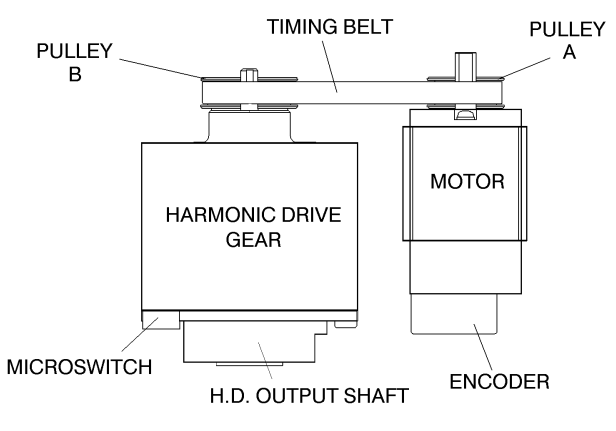
\includegraphics[scale=0.5]{img/cap2/scorbot_drive}
	\caption{Sistema de actuación usado en las articulaciones del robot Scorbot.}
	\label{cap2_scorbot_drive}
\end{figure}

La Tabla \ref{cap2_scorbot_specs} muestra las especificaciones de cada uno de las articulaciones del robot Scorbot. Mientras que la Table \ref{cap2_scorbot_motor_specs} muestra los parámetros de los motores usados en las articulaciones.

\begin{table}[]
	\begin{tabular}{|l|l|l|l|}
		\hline
		\multicolumn{1}{|c|}{\textbf{Parámetro}} & \multicolumn{1}{|c|}{\textbf{Símbolo}} & \multicolumn{1}{c|}{\textbf{Motor Pittman-9434}}     & \multicolumn{1}{c|}{\textbf{Motor Pittman-9413}}     \\ \hline
		Constante motor           & $k_m$ & $\SI{2.13e-2}{\frac{\newton\metre}{\sqrt{\watt}}}$ & $\SI{1.37e-2}{\frac{\newton\metre}{\sqrt{\watt}}}$ \\ \hline
		Constante torque          & $k_T$ & $\SI{3.65e-2}{\frac{\newton\metre}{\ampere}}$ & $\SI{3.95e-2}{\frac{\newton\metre}{\ampere}}$ \\ \hline
		Resistencia de armadura   & $R_a$ & $\SI{2.96}{\ohm}$ & $\SI{8.33}{\ohm}$ \\ \hline
		Inductancia de armadura   & $L_a$ & $\SI{2.51}{\milli\henry}$ & $\SI{6.17}{\milli\henry}$ \\ \hline
		Inercia del eje           & $J$   & $\SI{4.17e-6}{\kilogram\metre^2}$ & $\SI{2.8e-6}{\kilogram\metre^2}$ \\ \hline
		Coeficiente roce viscoso  & $B$   & $\SI{4.50e-4}{\frac{\newton\metre}{\radian\per\second}}$ & $\SI{1.9e-4}{\frac{\newton\metre}{\radian\per\second}}$ \\ \hline
	\end{tabular}
	\caption{Especificaciones de motores PMDC.}
	\label{cap2_scorbot_motor_specs}
\end{table}

\begin{table}[]
\centering
\begin{tabular}{|l|l|l|l|}
\hline
\multicolumn{1}{|c|}{\textbf{Eje}} & \textbf{Nombre} & \textbf{Rango} & \multicolumn{1}{c|}{\textbf{Especificaciones}} \\ \hline

{\multirow{5}{*}{1}} & \multirow{5}{*}{Base} & \multirow{5}{*}{\ang{310}} & Voltaje: \SI{12}{\volt} \\ \cline{4-4} 
\multicolumn{1}{|c|}{} &  &  & Motor Pittman-9434G697 \\ \cline{4-4} 
\multicolumn{1}{|c|}{} &  &  & Encoder HP-HEDS-5500-K11 (incremental) 96 pulsos/rev \\ \cline{4-4} 
\multicolumn{1}{|c|}{} &  &  & \textit{Harmonic drive} razón 1:160 \\ \cline{4-4} 
\multicolumn{1}{|c|}{} &  &  & \textit{Timing belt} razón 1:3 \\ \hline
\multirow{5}{*}{2} & \multirow{5}{*}{Shoulder} & \multirow{5}{*}{\ang{170}} & Voltaje: \SI{12}{\volt} \\ \cline{4-4} 
 &  &  & Motor Pittman-9434G697 \\ \cline{4-4} 
 &  &  & Encoder HP-HEDS-5500-K11 (incremental) 96 pulsos/rev \\ \cline{4-4} 
 &  &  & \textit{Harmonic drive} razón 1:160 \\ \cline{4-4} 
 &  &  & \textit{Timing belt} razón 1:3 \\ \hline
\multirow{5}{*}{3} & \multirow{5}{*}{Elbow} & \multirow{5}{*}{\ang{225}} & Voltaje: \SI{12}{\volt} \\ \cline{4-4} 
 &  &  & Motor Pittman-9434G697 \\ \cline{4-4} 
 &  &  & Encoder HP-HEDS-5500-K11 (incremental) 96 pulsos/rev \\ \cline{4-4} 
 &  &  & \textit{Harmonic drive} razón 1:160 \\ \cline{4-4} 
 &  &  & \textit{Timing belt} razón 1:3 \\ \hline
\multirow{5}{*}{4} & \multirow{5}{*}{Wrist pitch} & \multirow{5}{*}{\ang{180}} & Voltaje: \SI{12}{\volt} \\ \cline{4-4} 
 &  &  & Motor Pittman-9413G698 \\ \cline{4-4} 
 &  &  & Encoder HP-HEDS-5500-K11 (incremental) 96 pulsos/rev \\ \cline{4-4} 
 &  &  & \textit{Harmonic drive} razón 1:100 \\ \cline{4-4} 
 &  &  & \textit{Timing belt} razón 1:3 \\ \hline
\multirow{4}{*}{5} & \multirow{4}{*}{Wrist roll} & \multirow{4}{*}{\ang{360}} & Voltaje: \SI{12}{\volt} \\ \cline{4-4} 
 &  &  & Motor Pittman-9413G698 \\ \cline{4-4} 
 &  &  & Encoder HP-HEDS-5500-K11 (incremental) 96 pulsos/rev \\ \cline{4-4} 
 &  &  & \textit{Harmonic drive} razón 1:100 \\ \hline
\end{tabular}
\caption{Especificaciones de articulaciones robot Scorbot ER VII.}
\label{cap2_scorbot_specs}
\end{table}




\section{Conceptos de cinemática}

Una de las tareas principales de un robot manipulador corresponde a seguir una trayectoria dejando al efector en una posición deseada. En orden de mover el robot a través de dos o más puntos de una trayectoria objetivo en un tiempo, velocidad y aceleración especificados, es necesario definir el movimiento de cada uno de los componentes del robot.

El análisis cinemático es el estudio del movimiento de los distintos elementos del robot, sin considerar las fuerzas y momentos que producen tal movimiento de los elementos.

\subsection{Cinemática directa}

Cinemática directa es el nombre que recibe el problema de encontrar la posición y orientación del efector relativo a la base del robot dados todas posiciones de las articulaciones y parámetros geométricos de los elementos que constituyen el robot. Usualmente, el sistema de referencia fijo en el efector se denomina \textit{tool frame} \cite{handbook}.

En la práctica, la cinemática directa es resuelta notando que para una cadena de elementos en serie, como es el caso del robot Scorbot, la transformada entre el sistema de referencia y el sistema fijo en el efector esta dada por la concatenación de las transformadas entre elementos adyacentes de la cadena cinemática.

\begin{equation}
T_0^5(\vec{\theta}) = T_0^1 T_1^2 T_2^3 T_3^4 T_4^5 
\end{equation}

Donde $\vec{\theta}=[\theta_1,\dotsc,\theta_5]$, $\theta_i$ corresponde al ángulo de la articulación $i$-ésima y $T_j^i$ es la transformada homogénea del elemento $i$ con respecto al sistema de referencia $j$.

\subsection{Cinemática inversa}

Por otro lado, la cinemática inversa es el nombre que recibe el problema de encontrar el valor de las posiciones de las articulaciones dada la posición y orientación del efector.
Usualmente, el cálculo de la cinemática inversa involucra la resolución de sistemas geométricos complejos que dificulta la obtención de formas cerradas, en casos donde la forma cerrada no existe se pueden emplear métodos numéricos basados en el jacobiano del sistema.

La obtención de modelos exactos de cinemática directa e inversa es tratado de forma extensa en \cite{cole2007} y \cite{predescu2015}.

\section{Controladores PID}

Aunque las nuevas y eficaces teorías y metodologías de diseño de controladores se están desarrollando continuamente en el campo del control automático, los controladores Proporcional Integral Derivativo (PID) son todavía los controladores más ampliamente utilizados en la industria debido a la ventajosa relación costo-beneficio que pueden proporcionar. De hecho, aunque son relativamente simples de usar, son capaces de lograr un desempeño satisfactorio en muchas tareas de control de procesos. De hecho, su larga historia y el \textit{know-how} que se ha desarrollado a lo largo de los años lo ha consolidado como el controlador de retroalimentación estándar \cite{practical_pid}.

\subsection{Control proporcional}

Aplicar un controlador PID consiste en aplicar la suma de tres acciones de control: la acción proporcional, la acción integral y la acción derivativa. Estas acciones se describen a continuación.

\subsection{Control proporcional}
En control proporcional la acción de control es proporcional al error actual del sistema, como se muestra en la expresión (\ref{ctrl-kp}).

\begin{equation}\label{ctrl-kp}
u(t) = K_p e(t) = K_p(r(t)-y(t))
\end{equation}

Donde $K_p$ es la constante proporcional. El significado es directo, pues implementa la operación de incrementer la variable controlada cuando el error aumenta. La función de transferencia se muestra en la expresión (\ref{ctrls-kp}).

\begin{equation}\label{ctrls-kp}
C(s) = K_p
\end{equation}

\subsection{Control integral}

La acción interal es proporcional a la integral del error de control, es decir, esta dada por la expresión (\ref{ctrl-int-t}).

\begin{equation}\label{ctrl-int-t}
u(t)=K_i \int_{0}^{t}e(t)dt 
\end{equation}

Donde $K_i$ corresponde a la ganancia integral. Esta acción de control considera todos los valores pasados del error de control. La función de transferencia asociada esta dada por la ecuación ()
\begin{equation}\label{ctrl-int}
C(s)=K_i\frac{1}{s}
\end{equation}

La presencia de un polo en origen del plano complejo permite la reducción del error en estado estacionario ante una entrada o perturbación de tipo escalón. En otras palabras, la acción integral permite adaptar el valor de $u(t)$ de tal forma de alcanzar cero error en estado estacionario.

La aplicación conjunta de una acción proporcionar e integral da origen al controlador PI, ampliamente usado para resolver problemas oscilatorios de controladores On Off y error estacionario de controladores proporcionales. Si el control integral esta presente, el fenómeno de \textit{windup} puede ocurrir ante la presencia de saturación de la variable controlada.

\subsection{Control derivativo}

Mientras la acción de control proporcional esta basada en el valor actual del error de control y la acción integral esta basada en el los valores pasados del error de control, la acción derivativa esta basada en la predicción de los valores futuros del error de control. Una ley de control derivativa ideal se muestra en la expresión ().

\begin{equation}
u(t) = K_d \frac{de}{dt}
\end{equation}

Donde $K_d$ corresponde a la ganancia derivativa. La función de transferencia esta dada por la expresión ().
\begin{equation}
C(s) = K_d s
\end{equation}

Consideremos la expansión en serie de Taylor del error de control en $t + T_d$.

\begin{equation}
e(t + T_d) = e(t) + T_d \frac{de}{dt}
\end{equation}

Si aplicamos la ley de control proporcional a esta expresión se obtiene:

\begin{equation}
u(t) = K_p \left( e(t) + T_d \frac{de}{dt} \right)
\end{equation}

Esto corresponde naturalmente a un controlador PD. La variable controlada en $t$ esta también calculada usando una estimación del error de control en $t+T_d$. Por esta razón, se establece que el control derivativo añade elementos de control predictivo. Esto parece tener un gran potencial para mejorar el desempeño, sin embargo, existen algunos problemas en la implementación de este tipo de controladores, en especial las relacionadas con la amplificación del ruido de alta frecuencia.

\subsection{Discretización de controladores}

En la sección pasada se describió la función de los controladores PID continuos, gran parte de las aplicaciones de control actuales se realizan con ayuda elementos digitales, como microcontroladores o FPGA, por lo que los controladores deben ser llevados al dominio discreto para ser implementados en estas plataformas.

En términos de función de transferencia, buscamos una transformar la expresión en tiempo continuo $G(s)=\frac{B(s)}{A(s)}$ a una de tiempo discreto  $G(z)=\frac{B(z)}{A(z)}$, para lograr esto se debe encontrar la relación $s=f(z)$.

La relación $s=f(z)$ puede obtenerse considerando que para mantener estabilidad todos los polos del sistema deben ser mapeados dentro de la circunferencia unidad, de esta forma se obtiene que la relación (\ref{cap2_zmapping})\cite{oppenheim2009}.

\begin{equation}\label{cap2_zmapping}
z=e^{s T_s}
\end{equation}

Considerando una expansión de Taylor de primer orden sobre la expresión (\ref{cap2_zmapping}), se obtiene la expresión (\ref{cap2_tustin}), conocida como método de Tustin o bilineal.

\begin{eqnarray}
z &=& \frac{e^{s \frac{T_s}{2}}}{e^{-s \frac{T_s}{2}}}\\
z &\approx& \frac{1+s \frac{T_s}{2}}{1-s \frac{T_s}{2}} \label{cap2_tustin}.
\end{eqnarray}

De la expresión (\ref{cap2_tustin}) se puede obtener la relación (\ref{cap2_tustin_s}). Es común encontrar en literatura y documentación de DSP la notación $w=z^{-1}$.

\begin{eqnarray}
z &=& \frac{e^{s \frac{T_s}{2}}}{e^{-s \frac{T_s}{2}}}\\
z &\approx& \frac{1+s \frac{T_s}{2}}{1-s \frac{T_s}{2}} \label{cap2_tustin}.
\end{eqnarray}

\begin{equation}\label{cap2_tustin_s}
s \approx \frac{2}{T_s} \frac{1-z^{-1}}{1+z^{-1}} = \frac{2}{T_s} \frac{1-w}{1+w}
\end{equation}

\subsection{Implementación de controladores digitales}

Para describir la implementación de un controlador digital, consideremos un control integral, donde $k_i$ corresponde a la contante integral:

\begin{eqnarray}
C(s) &=& k_i \frac{1}{s}\\
C(s)_{s=\frac{2}{T_s} \frac{1-w}{1+w}} &=& \frac{k_i T_s}{2} \frac{1+w}{1-w} \\
C(w) &=& \frac{  \frac{k_i T_s}{2} w +  \frac{k_i T_s}{2} }{(-1)w+1} 
\end{eqnarray}

Considerando que un esquema de control realimentado, se tiene que $C(w) = \frac{u(w)}{e(w)}$, donde $u(w)$ corresponde a la salida del controlador y $e(w)$ al error, ambos en dominio discreto.

\begin{eqnarray}
\frac{u(w)}{e(w)} &=& \frac{  \frac{k_i T_s}{2} w +  \frac{k_i T_s}{2} }{(-1)w+1} \\
u(w)-u(w)w &=& e(w) \frac{k_i T_s}{2} w +  e(w) \frac{k_i T_s}{2} \label{cap2_eq_diff_w}
\end{eqnarray}

Aplicando transformada $Z$ inversa sobre la expresión (\ref{cap2_eq_diff_w}) se obtiene la ecuacion de diferencia:

\begin{eqnarray}
u(n)- u(n-1) &=&  \frac{k_i T_s}{2}(e(n)+e(n-1)) \\
\Delta u(n) &=& k_i \left( T_s \, \frac{e(n)+e(n-1)}{2} \right) \label{cap2_eq_control_int}
\end{eqnarray}

De la expresión \ref{cap2_eq_control_int}, muestra que el cambio en la salida del controlador esta dado por la integral del error. Notamos que podemos reescribir la ecuación de diferencia de la siguiente forma:

\begin{eqnarray}
u(n) &=&  \frac{k_i T_s}{2} e(n) + \alpha(n-1) \\
\alpha(n) &=& u(n) + \frac{k_i T_s}{2} e(n)
\end{eqnarray}

Esta representación nos indica que para implementar el controlador deseado solo se necesita almacenar un estado $\alpha(n)$, pues el corresponde a sistema de primer orden. La implementación en diagrama de bloques se muestra en la Figura \ref{cap2_block_integral}.

\begin{figure}[H]
  \centering
  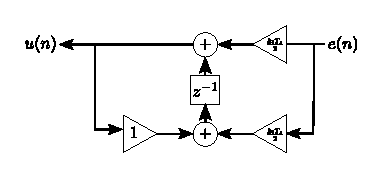
\includegraphics[scale=1.5]{img/cap2/block_pi}
  \caption{Diagrama de bloques controlador integral.}
  \label{cap2_block_integral}
\end{figure}

Esta represetación se denomina forma Directa II versión transpuesta, la cual es óptima con respecto a los elementos de retardo necesarios para la implementación, pues los polos y ceros comparten los elementos de retardo, lo que finalmente se traduce en el uso de una estructua de datos más compacta en el microcotrolador. De forma más general, la función de transferencia $H(w)$ de un filtro digital puede expresarse como muestra la expresión (\ref{cap2_filtro_digital}) y representarse en diagrama de bloques según la Figura (\ref{cap2_td2}).

\begin{equation}
H(w) = \frac{\sum_{k=0}^{M} b_k \, w^k}{1-\sum_{k=1}^{N} a_k \, w^k}\label{cap2_filtro_digital}
\end{equation}

\begin{figure}[H]
  \centering
  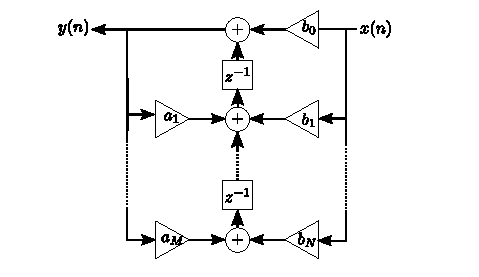
\includegraphics[scale=1.2]{img/cap2/tdf2}
  \caption{Diagrama de bloques para representación Directa II versión transpuesta.}
  \label{cap2_td2}
\end{figure}

\section{Motores de corriente continua}

El motor de corriente continua (CC) es la máquina eléctrica empleada en aplicaciones de potencia y tracción. Su sencillo accionamiento y estructura de control han permitido que siga vigente hasta nuestros días, a pesar de ser constructivamente más complejo que los que motores BLDC y requerir mantenimiento. Su velocidad fácilmente controlable y posibilidad de girar en ambos sentidos, lo  que permite aplicaciones de servo accionamientos y tracción.

El funcionamiento del motor de CC se basa en la fuerza generada por la interacción de un campo magnético inmóvil y uno generado por una bobina móvil (armadura), montada sobre un eje de rotación. La bobina móvil es alimentada a través de un sistema de escobillas y delgas para invertir la dirección de la corriente y, por consiguiente, el sentido del campo magnético generado, logrando que el torque resultante sea siempre favorable al sentido de giro \cite{vargas2006}. En la Figura \ref{cap2_motorcc} se muestra la bobina dentro de un campo magnético fijo de dirección horizontal.

\begin{figure}[H]
    \centering
    \begin{subfigure}[b]{0.48\textwidth}
            \includegraphics[width=\textwidth]{img/cap2/motor_cc1.png}
            \caption{Bobina elemental del motor de CC dispuesta sobre un eje de giro y alimentada a través de las escobillas.}
    \end{subfigure}
    ~
    \begin{subfigure}[b]{0.48\textwidth}
            \includegraphics[width=\textwidth]{img/cap2/motor_cc2.png}
            \caption{Bobina montada en un rotor dentro de un campo magnético fijo cuya dirección es perpendicular al eje de giro.}
    \end{subfigure}
    \caption{Bobinas del motor de CC}
    \label{cap2_motorcc}
\end{figure}


El flujo de campo $\phi_f$ de dirección fija generado por el estator puede ser producido por un devanado o imanes permanentes, como es el caso del los motores que posee el manipulador Scorbot ER-VII. El uso de imanes permanentes establece un flujo de campo $\phi_f$ constate, esto mejora la eficiencia de la máquina, pero limita la velocidad de operación de la misma, pues no es posible operar a flujo debilitado.

En un motor de CC, el par de torsión electromagnético $T_m$ es producto de la interacción entre el flujo de campo $\phi_f$ y la corriente de armadura $i_a$.

\begin{eqnarray}
T_m &=& k_f \phi_f i_a \\
T_m &=& k_T i_a
\end{eqnarray}

Donde $k_f$ es la constante de par de torsión del motor. Como $\phi_f$ es constante, se usa $k_T= k_f \phi_f$.

En el circuito del inducido se produce una fuerza contraelectromotriz por la rotación de conductores de inducido a una velocidad $\omega_m$ en la presencia de un flujo de campo $\phi_f$.

\begin{equation}
e_a = k_e \phi_f \omega_m
\end{equation}

Donde $k_e$ es la constante de voltaje del motor. Se puede demostrar \cite{mohan}, que usando unidades SI $k_e \phi_f = k_T$, de esta forma fuerza contraelectromotriz, también denominada reacción de armadura, esta dada por la Ecuación \ref{eq_reaccion_armadura}.

\begin{equation}\label{eq_reaccion_armadura}
e_a = k_T \omega_m
\end{equation}

En la práctica se aplica una fuente de voltaje controlable $v_t$ a los terminales de inducido para establecer una corriente de armadura $i_a$. Por tanto, la corriente $i_a$ en el circuito de inducido se determina por $v_t$, la fuerza contraelectromotriz $e_a$, la resistencia del devanado del inducido $R_a$ y la inductancia del devanado del inducido $L_a$ se ralacionan como muestra la Ecuación \ref{eq_armadura}, esta ecuación se ilustra como circuito equivalente en la Figura \ref{cap2_dc_motor}.

\begin{equation}\label{eq_armadura}
v_t = e_a + R_a i_a + L_a \dv{i_a}{t}
\end{equation}

La ecuación anterior determina el comportamiento eléctrico del motor de corriente continua, el comportamiento mecánico esta dado por la Ecuación \ref{eq_mecanica}, donde se ve la interacción del motor con la carga mecánica.

\begin{equation}\label{eq_mecanica}
T_m = T_l + B \omega_m + J \dv{\omega_m}{t}
\end{equation}

Donde $J$ y $B$ son la inercia y amortiguamiento equivalente total, respectivamente, de la combinación motor carga y $T_l$ es el par de torsión de trabajo equivalente de la carga.

\begin{figure}[H]
  \centering
  \includegraphics[scale=0.3]{img/cap2/dc_motor_circuit}
  \caption{Circuito equivalente de un motor de corriente continua.}
  \label{cap2_dc_motor}
\end{figure}

Un hecho importante de la actuación robot manipuladores corresponde a la naturaleza dinámica de la carga mecánica de cada articulación actuada, esto debido efectos gravitatorios y dinámicos generados por otros enlaces en movimiento de la cadena cinemática.


\subsection{Control de motores de corriente continua}

Como se mostró anteriormente, el torque producido por el motor de CC es proporcional a la corriente de armadura, dado que el objetivo es el control de las variables mecánicas (\textit{i.e.} torque, velocidad) es directo establecer como primera estructura el control la corriente de armadura. Para el control de la corriente de armadura es necesario que $v_t$ esté conectado a una fuente de voltaje controlable, esto se logra utilizando un circuito llamado convertidor de puente completo o puente H, el cual utiliza una estructura de puente que permite la conducción en ambos sentidos, tal como se muestra en la Figura \ref{cap2_punteh}.

\begin{figure}[ht]
  \centering
  \includegraphics[scale=.2]{img/cap2/puenteh}
  \caption{Configuración del puente H.}
  \label{cap2_punteh}
\end{figure}

El uso de modulación PWM en el encendido de los transistores permite controlar el valor efectivo de la tensión de alimentación del motor CC. El diseño de estos dispositivos de potencia es un trabajo complejo, pues requiere la correcta elección de semiconductores, un \textit{layout} capaz de soportar altas corrientes y evitar la aparición de inductancias parásitas.

Dada la naturaleza inductiva del circuito de armadura, la modulación PWM de la tensión no establece un régimen de corriente pulsante, si no cierto nivel de rizo en la corriente estableciendo un estado que se denomina de corriente plana. Si el motor posee una baja inductancia de armadura, es posible que salga del régimen de corriente plana y se produzcan torques pulsantes. Este efecto puede ser reducido aumentando la frecuencia de conmutación o la conexión de inductancias en serie.

Afortunadamente, dado la gran demanda de estos dispositivos por parte de la industria automovilística, fabricantes de semiconductores entregan soluciones acorde a los requerimientos.

\section{Interfaces hápticas}

Los dispositivos hápticos son capaces de proporcionar una retroalimentación de fuerza al usuario que lo emplea, de esta forma complementan sistemas de operación visuales al entregar más información al operador. Esta tecnología puede aplicarse a múltiples sectores con el fin de facilitar su ejecución: medicina, realidad virtual, modelado, robótica, entre otras.

\subsection{Phantom Omni \texttrademark}

Phantom Omni \texttrademark (actualmente Geomatic\textregistered \, Touch \texttrademark) es un dispositivo háptico de seis grados de libertad (6 \textit{DOF}) desarrollado por Sensable\textregistered, permite leer la posición de sus seis articulaciones y posee tres actuadores conectados a los tras primeras articulaciones, permitiendo la aplicación de fuerzas, que solo pueden controlar la posición del \textit{stylus} en el espacio cartesiano.

\begin{figure}[ht]
  \centering
  \includegraphics[scale=.2]{img/cap2/phantom_omni}
  \caption{Phantom Omni \texttrademark.}
  \label{cap2_phantom}
\end{figure}

Un aspecto importante del diseño es el desacople entre la posición y orientación \cite{beckman2007}, las tres primeras articulaciones son usadas para posicionar el \textit{stylus} y las restantes establecen la orientación del mismo. Los ejes de giro de estas últimas tres articulaciones se intersectan en un mismo punto, por lo que se puede interpretar como una articulación esférica.

La configuración cinemática del Phantom Omni \texttrademark \, es similar a la del robot Scorbot ER VII, pues poseen una cadena cinemática con una base, dos elementos articulados que se mueven en un plano y una muñeca. La mayor diferencia entre ellos, aparte de su tamaño, radica en que el dispositivo háptico posee 6 grados de libertad y solo tres articulaciones son actuadas, por otro lado el robot posee solo 5 grados de libertad, todos ellos actuados. 

\section{Bus de campo}

Los primeros enlaces de datos estaban limitados a la conexión entre dos dispositivos, esto se traducía en que cada nuevo dispositivo debía ser conectado directamente al controlador en una topología de estrella. Esto llevó al desarrollo de buses de campo (\textit{fieldbuses}), definidos en el estándar IEC 61158, permitiendo la conexión múltiples nodos usando el mismo cable, lo que se denomina \textit{multidrop bus}. Esto trajo consigo cableados más simples y redes más modulares. Compartir un bus entre varios nodos requiere de un protocolo que maneje de forma adecuada el envío y recepción de datos de los dispositivos conectado al bus.

Un esquema de control distribuido requiere de un bus de campo capaz de compartir información con los dispositivos de forma determinista, pues los algoritmos de control e información critica deben cumplir estrictos requerimientos temporales (\textit{timming}). Algunos requerimientos clásicos se describen a continuación:

\begin{itemize}

\item Frecuencia de actualización: Controladores obtienen información de sensores y envían comandos a los actuadores de manera periódica, usualmente, a una frecuencia fija. Esta frecuencia depende de la aplicación en particular, por ejemplo es usual que lazos de control de servomotores tengan frecuencias de actualización cercanas a \SI{1}{kHz}.

\item \textit{Jitter}: Corresponde a la variabilidad temporal durante el envío de señales digitales. La presencia de \textit{jitter} en el bus de campo puede tener efectos no deseados, siguiendo el ejemplo anterior, un \textit{jitter} de \SI{1}{\milli\second} puede considerarse inaceptable, pues es del orden del tiempo de actualización.

\end{itemize}


\subsection{EtherCAT}

EtherCAT (\textit{Ethernet for Control Automation Technology}) es un bus de campo de código abierto, fue creado con el fin de emplear el potencial Ethernet y mejorar las áreas donde este falla al momento de implementarse en redes de control, de esta forma introduce comportamiento determinista y reducción en el tiempo de procesamiento de paquetes de datos pequeños.

\subsubsection{Estructura maestro-esclavo}

EtherCAT emplea una estructura maestro-esclavo donde cada dispositivo es conectado en cadena uno tras otro como se muestra en la Figura \ref{cap2_ethercat_chain}.

La transmisión es iniciada por el dispositivo maestro, el mensaje es transmitido a la cadena de esclavos donde cada dispositivo puede leer o escribir en el mensaje antes de pasarlo al siguiente dispositivo. Una vez el mensaje alcanza el último dispositivo esclavo, éste lo envía hacia el maestro a través de la cadena. Desde fuera, de la estructura formada por la cadena de esclavos se puede considerar como un nodo Ethernet.

\begin{figure}[ht]
  \centering
  \includegraphics[scale=.5]{img/cap2/ethercat_chain}
  \caption{Estructura maestro esclavo de EtherCAT.}
  \label{cap2_ethercat_chain}
\end{figure}

\subsubsection{Enlace de datos}

Dado que cada dispositivo esclavo debe leer el mensaje antes de saber que hacer con él, este proceso puede introducir una cantidad de calculo que debe realizar el software y que va en desmedro del rendimiento aplicación principal. Para evitar eso cada esclavo esta equipado con \textit{EtherCAT Slave Controller} (ESC), el cual procesa el mensaje recibido en hardware, reduciendo de forma significativa el tiempo de procesamiento en el esclavo. Gracias a esto, el dispositivo esclavo empieza la transmisión al siguiente nodo cuando aún esta recibiendo el mensaje. El ESC contiene toda la funcionalidad de la capa de enlace de datos especificada por el estándar, la capa de aplicación depende del tipo de ESC usada.

Dado el enlace de datos se realiza por hardware, los dispositivos esclavos deben contar con hardware especializado para usar el bus de campo EtherCAT. Usualmente existen dos alternativas para la integración de EtherCAT en un dispositivo: uso de un EtherCAT ASIC o integración de un IP usando una FPGA. Actualmente, esta tecnología se integra en microcontroladores, permitiendo diseños más compactos y económicos (Figura \ref{cap2_ethercat}).

\begin{figure}[H]
  \centering
  \begin{subfigure}[b]{0.4\textwidth}
    \includegraphics[width=0.6\textwidth]{img/cap2/ethercat_asic.png}
    \caption{EtherCAT ASIC de Beckhoff Automation GmbH.}
    \end{subfigure}%
    ~
  \begin{subfigure}[b]{0.4\textwidth}
    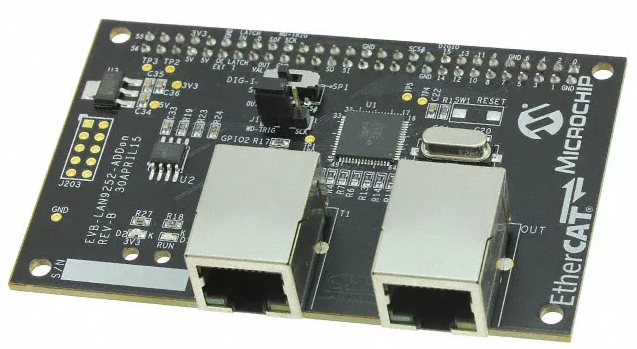
\includegraphics[width=\textwidth]{img/cap2/microchip_lan9252}
    \caption{Placa de desarrollo del microcontrolador LAN9252 de Microchip puerto EtherCAT integrado}
    \end{subfigure}
  \caption{Alternativas de integración de EtherCAT en dispositivos.}
  \label{cap2_ethercat}
\end{figure}

\section{Componentes de software}

\subsection{ROS}

Robot Operating System (ROS) \cite{quigley2009} es un  framework para el desarrollo de aplicaciones robóticas, ofrece herramientas, librerías, abstracción de hardware, controladores de dispositivos, visualizadores, comunicación entre procesos, gestión de paquetes, entre otros.

A pesar de su nombre, ROS no es un sistema operativo propiamente dicho, es más bien un middlewere que se integra en sistemas GNU/Linux como Ubuntu. Una de sus principales ventajas es su amplia comunidad y que se encuentra bajo la licencia BSD, que permite el uso del software en aplicaciones comerciales. Fue desarrollado en 2007 por el Laboratorio de Inteligencia Artificial de Stanford bajo el nombre de \textit{switchyard}, luego su desarrollo continuó en el laboratorio de investigación robótico Willow Garage, actualmente la OSRF (\textit{Open Source Robotics Foundation}) es la encargada de mantener las herramientas básicas de ROS.

Uno es los aspectos más importantes de ROS es interfaz para la comunicación entre procesos. Un nodo, unidad de software básica en ROS, puede publicar o suscribirse a un tópico. En este tópico se escriben/leen mensajes que han sido depositados por otros nodos. Puede haber varios publicadores y subscriptores sobre el mismo tópico concurrentemente. Un único nodo puede publicar y subscribiese a múltiples tópicos.

Los mensajes son estructuras de datos que soportan tipos primitivos como
enteros, punto flotante, arreglos de primitivas y constantes. Adicionalmente los mensajes pueden estar compuestos por otros mensajes y por arreglos de mensajes, dando la profundidad que se requiera.

Otro elemento primordial lo constituyen los servicios, estos se definen mediante un par de mensajes, unos para la solicitud (\textit{request}) y otro para la respuesta (\textit{response}). Un nodo ofrece un servicio bajo un nombre y un cliente llama al servicio enviando un mensaje de solicitud y esperando a la respuesta.

\section{Evaluación del sistema}

Para la evaluación del sistema se propone el uso de una aplicación de teleoperación háptica donde operador podrá:

\begin{itemize}

\item Mover de forma continua el robot manipulador usando la interfaz hápica Phantom Omni \texttrademark.
\item Obtener \textit{feedback} hápico considerando variables internas del robot, como la posición actual.
\item Interactuar de forma hápitica con objetos, previamente definidos, en el espacio de trabajo del robot.

\end{itemize}

\chapter{Diseño}

El robot Scorbot cuenta con una unidad de control propietaria que permite movimiento por ejes y cartesiano a través de un \textit{teach pendant}. También puede ser conectado a un ordenador mediante puerto serial, para el envía de posiciones y trayectorias predefinidas. Lamentablemente el software de control ha quedado obsoleto, pues solo era compatible con MS-DOS, limitando el uso del dispositivo.

Esta limitaciones abren la puerta para el desarrollo de un hardware y software de control del robot, esta vez de basado en herramientas de código libre y estándares industriales que garanticen una mayor vigencia. Además, hacer que el hardware y software del robot sean compatibles con \textit{frameworks} de robótica, reduce el tiempo y dificultad en tareas de integración y creación de nuevas aplicaciones, mejorando su posibilidad de uso futuro.

\section{Controladores} \label{cap3_controladores}

La función principal de los controladores es el manejo del movimiento de un motor DC. Para realizar esta tarea el controlador debe contar con un microcontrolador, encargado de realizar las tareas de computo y comunicación, y una etapa de potencia, quien transfiere al motor los comandos.

Se consideró que los nuevos controladores fueran capaces de, al menos, tener el mismo desempeño que los originales, de esta forma se establecen una serie de requerimientos:

\begin{itemize}
\item Esquema de control distribuido, cada uno de las articulaciones del robot será controlada de forma independiente por un un controlador.
\item Sistema de comunicación capaz de soportar una frecuencia de actualización de 1 \si{\kilo\hertz}.
\item Microcontrolador capaz de establecer un control de corriente a una frecuencia de 10 \si{\kilo\hertz}.
\item La etapa de potencia debe ser capaz de controlar motores DC de 12 \si{\volt} con un consumo \textit{peak} de 8 \si{\ampere}. La frecuencia de conmutación debe ser al menos de 20 \si{\kilo\hertz}, para reducir el rizado de corriente y quede fuera del rango audible. 
\end{itemize}

\subsection{Sistema de comunicación}

Dado que cada articulación del robot esta constituida por los mismos elementos, parece natural replicar el sistema de control en cada una ellas y establecer sistema de control distribuido. De esta forma, cada una de las articulaciones de controla de forma independiente por un hardware dedicado, denominado esclavo (\textit{slave}). Todos los controladores esclavos son conectados usando un bus de datos con dispositivo maestro (\textit{master}) que establece las referencias de cada controlador.

Uno factor importante en el control distribuido es el tipo de comunicación usado, los principales requerimientos para el bus de campo son:
\begin{itemize}
\item Conexión por topología \textit{daisy chain}
\item Protocolo abierto
\item Rápida transmisión de datos y bajo \textit{jitter} 
\item Minimizar el uso de hardware especializado
\end{itemize}

Dados estos creiterios, según \cite{liu2015} el bus de campo EtherCAT el indicado para el diseño de controladores modulares para articulaciones, pues es corresponde a un bus de campo rápido, capaz de alzanr tasas de hasta \SI{100}{Mbit/s} y posee mecanismos de sincronización con una exactitud cercana a los \SI{25}{\nano\second}.

\subsubsection{Uso de librerías de Ethercat}

SOEM
Flanders Mechatronics Technology Centre has decided to release their EtherCAT PR2
Ig gmbh

\subsection{Microcontrolador}

La familia de microcontroladores XMC4 de Infineon Technologies AG esta especilizada para tareas de control de motores y comunicación industrial, por lo que integran hardware especifico para realizar esta tareas. De esta forma, el microcontrolador escogido corresponde al XMC4800, microcontrolador con núcleo ARM Cortex M4 con unidad de punto flotante, incorpora una serie de perifericos útiles utiles para el desarrollo de sistema de control, \textit{timers} de alta resolución para generación de PWM, interfaz para lectura de encoders (POSIF) y módulo comunicación EtherCAT integrado. La Figura \ref{cap3_xmc4800_data} muestra los distintos módulos que posee el XMC4800.

\begin{figure}[ht]
  \centering
  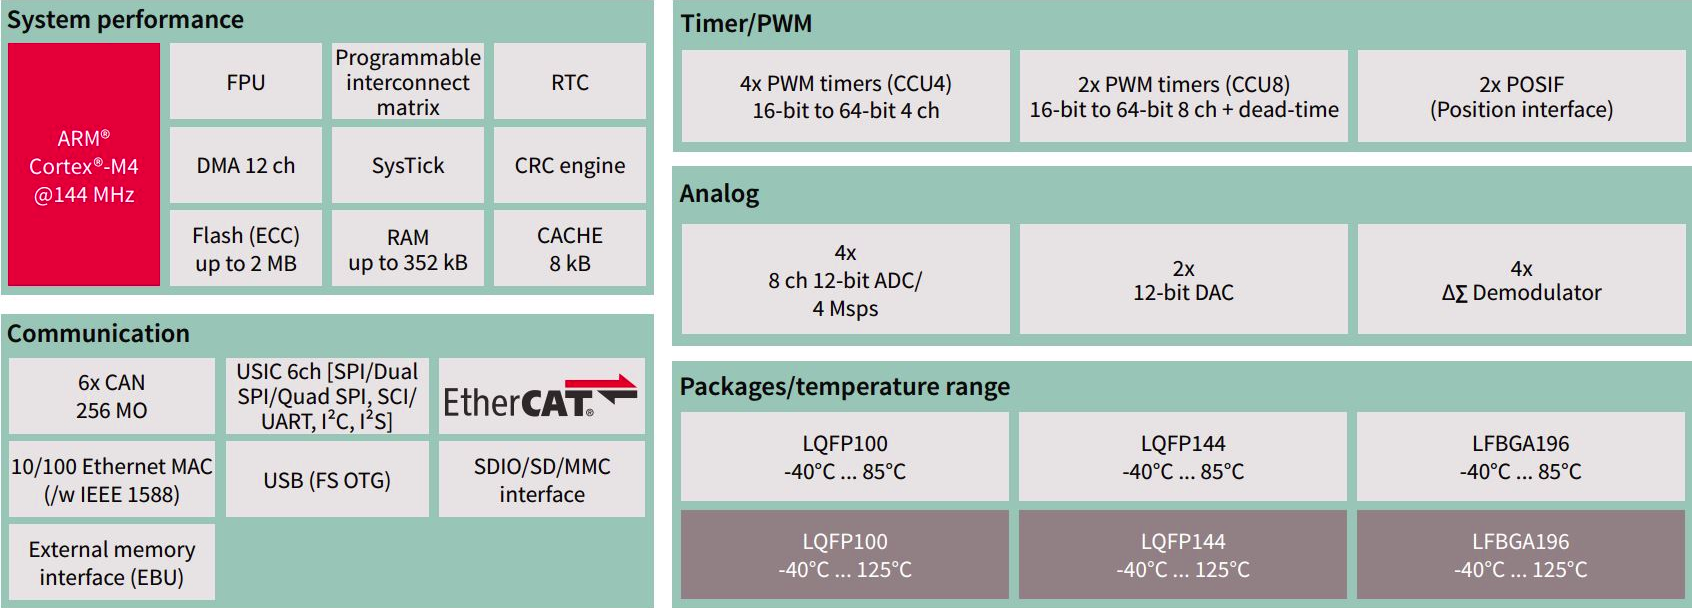
\includegraphics[scale=.2]{img/cap3/xmc4800_data}
  \caption{Carácteristicas del microcontrolador XMC4800. MO: Message Objects, Msps: Mega samples per second.}
  \label{cap3_xmc4800_data}
\end{figure}

La configuración de perifiericos en este tipo de microcontroladores suele ser una tarea compleja, dada las distintos \textit{pin out} y configuraciones de cada uno. Afortunadamente, el fabricante provee un IDE llamado Dave (Digital Application Virtual Engineer) que posee herramientas de generación de código a partir de una interfaz gráfica.

Otra carácteristica importante es que la placa de desarrollo escogida de este microcontrolador, la XMC4800 Relax EtherCAT Kit (Figura \ref{cap3_xmc4800}), posee la mayoría de componentes externos necesarios para el uso de las distintas funcionalidades del microcontrolador, como dos Ethernet PHY (transceiver) para la comunicación EtherCAT. Además integra un programador y debugger Segger J-Link que permite establecer \textit{break points} en el código y acceder a distintos registros de microcontrolador en tiempo real.

\begin{figure}[ht]
  \centering
  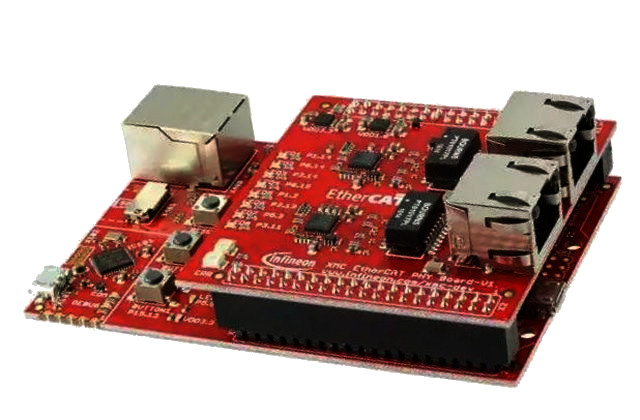
\includegraphics[scale=.4]{img/cap3/xmc4800}
  \caption{Placa de desarrollo XMC4800 Relax EtherCAT Kit.}
  \label{cap3_xmc4800}
\end{figure}
 

\subsection{Puente H}

Para la etapa de potencia se selecciono un puente H basado en el IC BTN8982TA, el cual corresponde a un \textit{half bridge} de alta corriente para aplicaciones con motores, contiene 
un MOSFET canal P para el \textit{high-side} y un canal N para el \textit{low-side}, ambos con un driver integrado, que permite su disparo directo desde un microcontrolador.

Para implementación se uso la placa de desarrollo \textit{Motor Control Shield}, que usa dos BTN8982TA en una configuración \textit{full bridge}, una imagen referencial se muestra  en la Figura \ref{cap2_punteh_infineon}, las principales carácteristicas:

\begin{itemize}
\item Control bidireccional de motor DC con escobillas de hasta \SI{250}{\watt} continuos.
\item Rango de tensión de entrada nominal \SI{8}{\volt} a \SI{18}{\volt} (\SI{6}{\volt} a \SI{40}{\volt} máximo).
\item Corriente máxima \SI{30}{\ampere}, restringida por la disipación del PCB (BTN8982TA tiene un limite de \SI{55}{\ampere}).
\item Frecuencia de conmutación hasta \SI{30}{\kilo\hertz}.
\end{itemize}

\begin{figure}[ht]
  \centering
  \includegraphics[scale=.35]{img/cap2/puenteh_infineon}
  \caption{Puente H fabricado por Infineon Technologies AG\textregistered \, basado en BTN8982TA.}
  \label{cap2_punteh_infineon}
\end{figure}

\subsection{Sensor de corriente}

Para la etapa de control del motor del motor de corriente continua es necesario contar con un sensor de corriente. Existen diversas tecnologías y técnicas de medición de corriente disponibles.

En el desarrollo de este trabajo se consideró el uso de un sensor de efecto hall Infineon TLI4970, su principal característica corresponde a la integración del ADC, DSP y acondicionamiento de señal se encuentran dentro del mismo \textit{package} \cite{infineonTLI4970}. Esto reduce la cantidad de elementos externos necesarios para realizar la medición de corriente. La Figura \ref{cap3_tli4970}, muestra el diagrama de bloques de los elementos internos del sensor.

\begin{figure}[H]
  \centering
  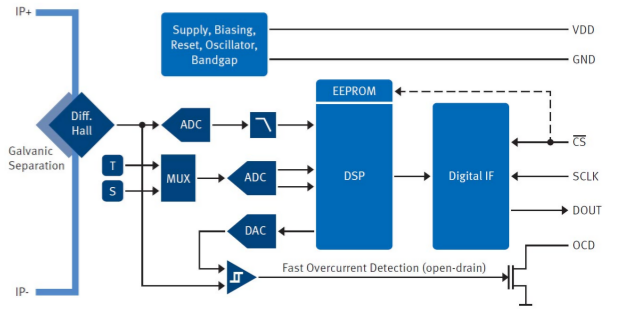
\includegraphics[scale=.45]{img/cap3/tli4970}
  \caption{Diagrama del sensor de corriente TLI4970.}
  \label{cap3_tli4970}
\end{figure}

El sensor tiene un rango máximo \SI{\pm 25}{\ampere} y una resolución de 10 bits. La salida del sensor se obtiene usando el protocolo SPI conectado directamente al microcontrolador.

\section{Integración de hardware}

Con el fin de reducir el tiempo de desarrollo, se consideró el uso de placas de desarrollo que provee el fabricante, de esta forma se usó directo el kit del microcontrolador XMC4800 y el puente H basado en el BTN8982TA. Para lograr una integración de hardware modular se considero el diseño de una PCB que permitira el montaje de los kits y otros componentes usados.

\subsubsection{PCB}

El diseño del PCB contempla la interconexión de las placas de desarrollo, el sensor de corriente TLI4970 




\chapter{Implementación}


\section{Controladores}

El controlador digital presentado en la sección \ref{cap3_controladores} se implementó en lenguaje C usando la transformada directa II.

%https://www.keil.com/pack/doc/CMSIS/DSP/html/group__BiquadCascadeDF2T.html


\subsection{Microcontrolador}



\subsection{Puente H}

Funciones especificas

\section{Integración de hardware}

Esquematico y componentes

\subsubsection{PCB}

Placa PCB

\section{Bus de campo}

Conexión


\section{Software}

\subsection{ROS}

Como se monstró en el capitulo pasado, su utilizó ROS como framework para realizar la integración. Los dispositivos de hardware, el robot Scorbot y el dispotivo háptico Phantom, cuentan con su \textit{nodo driver} que permiten la integración con el ecosistema ROS.

Se entiende por \textit{nodo driver} o ROS \textit{wrapper}, a una aplicación que actua como puente entre un dispositivo fisico y su representación en ROS, permitiendo interactuar de forma transparente con el dispositivo mediante el uso tópicos y servicios. Usualmente el \textit{nodo driver} hace uso de librerías proveidas por el fabricante o terceros para el manejo protocolos especificos del dispositivo. Por ejemplo, las siguientes aplicaciones cumplen esta función:

\begin{itemize}

\item \textit{ROSARIA}\cite{rosaria}: corresponde a una aplicación construido usando la librería \textit{Adept MobileRobots Robotics Interface for Applications} (ARIA), permite el control de robots móviles de las compañias Adept MobileRobots, MobileRobots Inc., y ActivMedia, por ejemplo el Pioneer 3-DX y 3-AT.

\item \textit{kinova-ros}\cite{kinova}: Es el driver oficial ofrecido por Kinova robotics para el uso de los robot manipuladores Jaco y Mico.

\end{itemize}

\subsubsection{Integración del robot Scorbot}

En esta sección se describirá la función de cada uno de los nodos que integran el software desarrollado para el control del robot Scorbot.

\begin{figure}[ht]
  \centering
  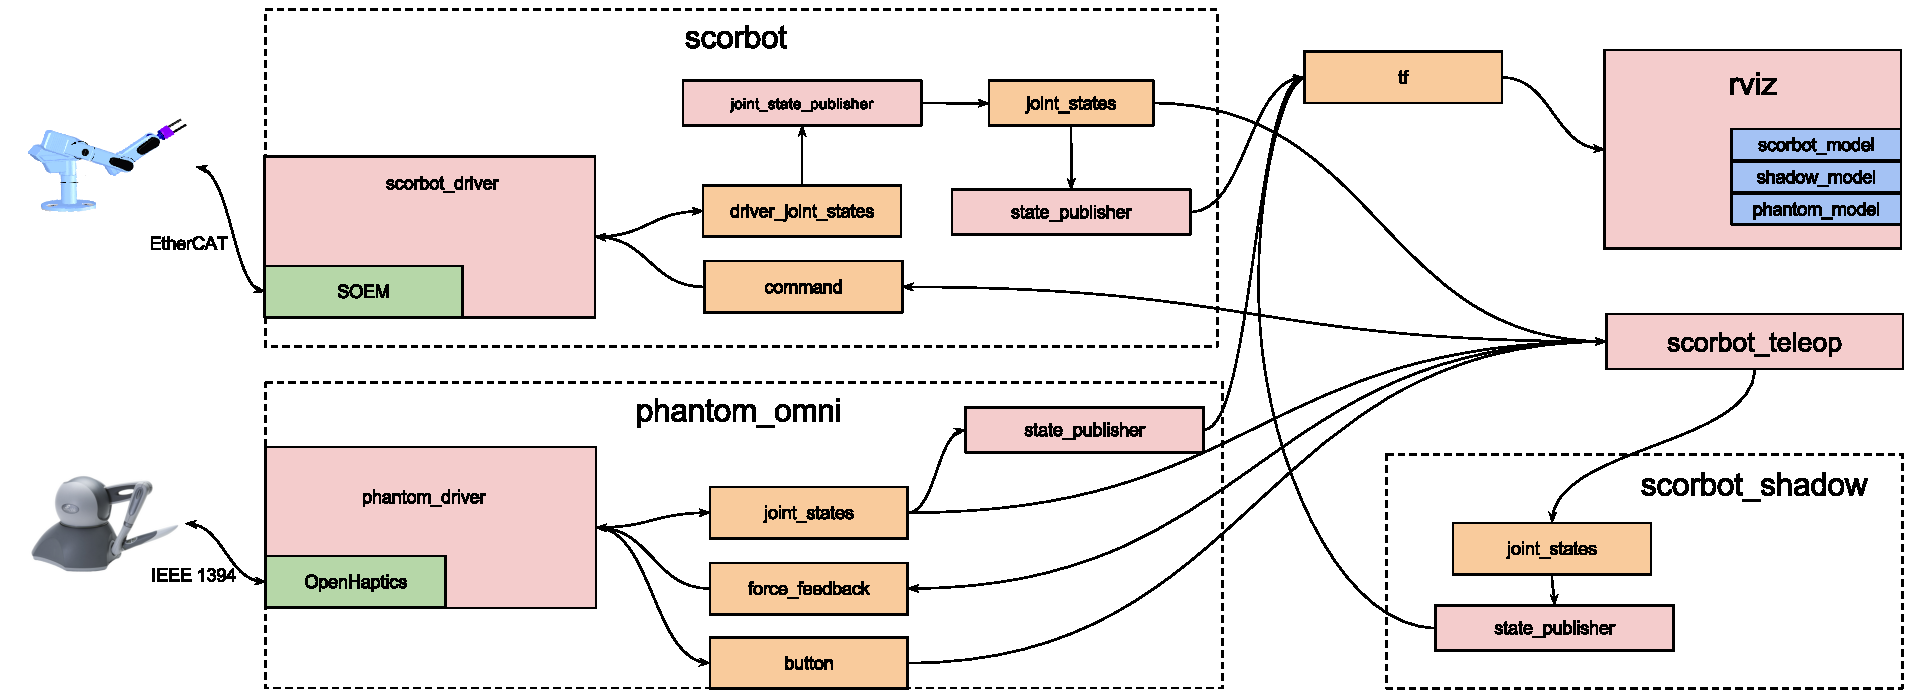
\includegraphics[width=\textwidth]{img/cap4/scorbot_software.pdf}
  \caption{Diagrama de nodos y tópicos de la aplicación.}
  \label{cap4_scorbot_software}
\end{figure}

\begin{description}

\item[\texttt{scorbot\_driver}] Corresponde al \textit{nodo driver} se integra con la librería SOEM \cite{soem} para la comunicación EtherCAT. Dado que este nodo ejecuta un ciclo de control, se consideraron una serie de requerimientos, muchos de ellos básicos para software de ejecución en tiempo real:

\begin{itemize}
\item Separación de hilos de ejecución, todas las tareas realacionadas con actualización de datos en el bus de control se realiza en un hilo independiente (\textit{control thread}) a las comunicaciones con el framework ROS (ROS \textit{thread}).
\item La comunicación entre el  \textit{control thread} y el ROS \textit{thread} se realiza usando estructuras de datos no bloqueantes.
\item La memoria utilizada por el hilo de control queda fija luego de la inicialización, de esta forma no se hacen llamados al sistema para pedir o liberar memoria.
\end{itemize}

SOEM mapea en memoria los dispositivos, es decir, desde el la aplicación master se tiene acceso a un buffer de memoria que permite leer y escribir en los dispositivos esclavos. Para obtener los datos manipulables, se debe usar la misma estructura de datos que usa el dispositivo esclavo para representar la información. \texttt{setpoint\_t} es la estructura usada como referenca (\textit{set point}), miestras que \texttt{joint\_data\_t} es la información del estado del controlador. Estas estructuras estan contenidas en un archivo de cabezera generado por el SSC, su modificación debe realizarse de forma cuidadosa, pues se pueden obtener errores de representación. El Código fuente \ref{cap4_estructuras} muestra la composición de ambas estructuras, notar el uso de la instrucción \texttt{PACKED}, que indica al compilador no añadir bytes entre los elementos de la estructura, de esta forma todos los elementos estan contiguos en memoria.

\begin{lstlisting}[language=C,style=csstyle, caption=Estructuras de datos usadas para mapear datos de dispositivos esclavos, label=cap4_estructuras]
typedef struct PACKED {
    uint16_t controlRegA;
    uint16_t controlRegB;
    int16_t  currentRef;
    int16_t currentLim;
    uint16_t pidCurrentKp;
    uint16_t pidCurrentKi;
    uint16_t pidCurrentKd;
} setpoint_t;

typedef struct PACKED {
    int16_t encPosition;
    int16_t encSpeed;
    int16_t current;
    uint16_t limits;
} joint_data_t;
\end{lstlisting}

Luego de realizar el mapeo en memoria, se creó la clase \texttt{ScorbotJointDriver}, encargada de representar cada controlador. Posee metodos para modificar la referencia y obtener el estado del controlador. Todos los controladores se agrupan en la clase \texttt{ScorbotHardwareInterface}, la cual abstrae las funciones del robót manipulador, como enviar una referencia a todas las articulaciones y detener todos los controladores. Es también encargada de ejecutar el ciclo de actualización de todos los controladores, este ciclo se ejecuta a \SI{1}{\kilo\hertz}.

ROS posee el paquete \texttt{ros\_control}, cuya función es facilitar la integración de dispositivos de control en ROS. De esta forma la clase \texttt{ScorbotHardwareInterface} hereda de \texttt{hardware\_interface::RobotHW} permitiendo la integración con \texttt{ros\_control}. El principal elemento utilizado de \texttt{ros\_control} correponde al \texttt{cotroller\_manager} una clase encargada de la comunicación entre \texttt{hardware\_interface::RobotHW} y tópicos ROS usando estructuras no bloqueantes en un hilo de ejecución independiente.

\begin{figure}[ht]
  \centering
  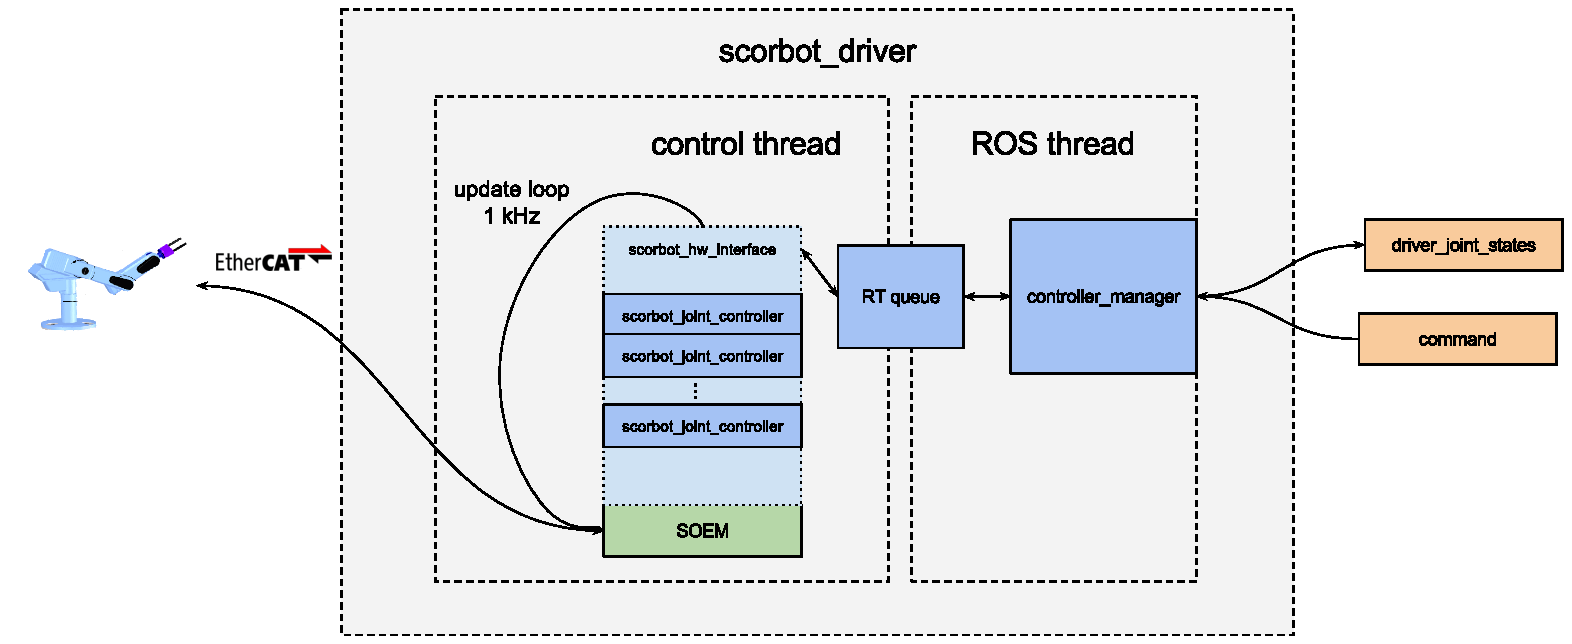
\includegraphics[width=\textwidth]{img/cap4/scorbot_driver.pdf}
  \caption{Diagrama del nodo \texttt{scorbot\_driver}.}
  \label{cap4_scorbot_driver}
\end{figure}

La Figura \ref{cap4_scorbot_driver} muestra la estructura del nodo \texttt{scorbot\_driver} como se ha señalado anteriormente. Como se ha mensionado anteriormente, es el \texttt{controller\_manager} quien se encarga de la comunicación con ROS, usando distintos tópicos:

\begin{itemize}

\item \texttt{driver\_joint\_states}: Contiene la información sobre el estado de cada articulación: posición, velocidad, aceleración y tiempo. Usa el mensaje  \texttt{sensor\_msgs/JointState[]}.

\item  \texttt{command}: Se usa para obtener la referencia de posición que será enviada a los controladores, se usa el mensaje \texttt{std\_msgs/Float64[]}.
 
\end{itemize}



\item[\texttt{joint\_state\_publisher}] Corresponde a un nodo estándar de ROS, cuya función es obtener los estados de las articulaciones de distintas fuentes (tópicos) y publicarlos de forma conjunta, completando el estado de todas las articulaciones dependiendo de la descripción del robot (URDF).

\item[\texttt{robot\_state\_publisher}] Corresponde a un nodo estándar de ROS, es el encargado de tomar la información de las articulaciones del robot y publicar el árbol de transformadas de cada uno de los enlaces del robot basado en la descripción del robot (URDF), es decir, ejecuta la cinemática directa del robot. Esta información de las transformadas es publicada en el tópico \texttt{/tf}.

\end{description}


\subsubsection{Integración de la interfaz Phantom Omni}

En esta sección se describirá la integración del dispositivo Phantom Omni en ROS. En este caso se hace uso del paquete \textit{phantom\_omni}\cite{phantom_git}, que contiene el ROS wrapper y URDF. La integración del Phantom Omni en ROS es similar a la realizada con el robot Scorbot, pues cuenta con el  ROS wrapper y los nodos \texttt{robot\_state\_publisher} y  \texttt{joint\_state\_publisher}, que cumplen la misma función descrita anteriormente, salvo que actúan sobre el estado del Phantom Omni.

\texttt{phantom\_driver} Corresponde al \textit{nodo driver} se integra con la librería OpenHaptics para la comunicación con dispositivo Phantom Omni a través de FireWire. Provee los siguientes tópicos:

\begin{itemize}
\item \texttt{joint\_states}: Información sobre el estado de las articulaciones usando el mensaje \\ \texttt{sensor\_msgs/JointState[]}.

\item \texttt{button}: Información sobre el estado de los botones del stylus del Phantom Omni, usando el mensaje \texttt{omni\_msgs/OmniButtonEvent}.

\item \texttt{force\_feedback}: El nodo se suscribe a éste tópico, al publicar en él el dispositivo aplica un par sobre las articulaciones actuadas.
\end{itemize}

Todos los tópicos del \texttt{phantom\_driver} se ejecutan a una frecuencia de \SI{100}{\hertz}, esto asegura que la referencia y retroalimentación hacia el operador sea adecuada, en terminos de retardo.


\subsubsection{Teleoperación}

La aplicación encargada de la teleoperación debe, básicamente, conectar el robot Scorbot con la interfaz háptica Phantom Omni, por conectar se entiende que la aplicación realiza el mapeo de las articulaciones del Phantom Omni hacia las articulaciones del Scorbot y entrega retroalimentación usando el Phantom Omni. Esta tarea es realizada por el nodo \texttt{scorbot\_teleop}.

El nodo \texttt{scorbot\_teleop} no controla directamente al robot Scorbot, si no que a un robot virtual, denominado Scorbot \textit{shadow}, esta representación almacena la posición deseada para el robot. Uno de los botones del \textit{stylus} del Phantom Omni actúa como gatillo, enviando la referencia es enviada al robot. Si el usuario mantiene el botón presionado, el software enviará de manera continua (\SI{100}{\hertz}) la referencia al robot.

\begin{figure}[H]
  \centering
  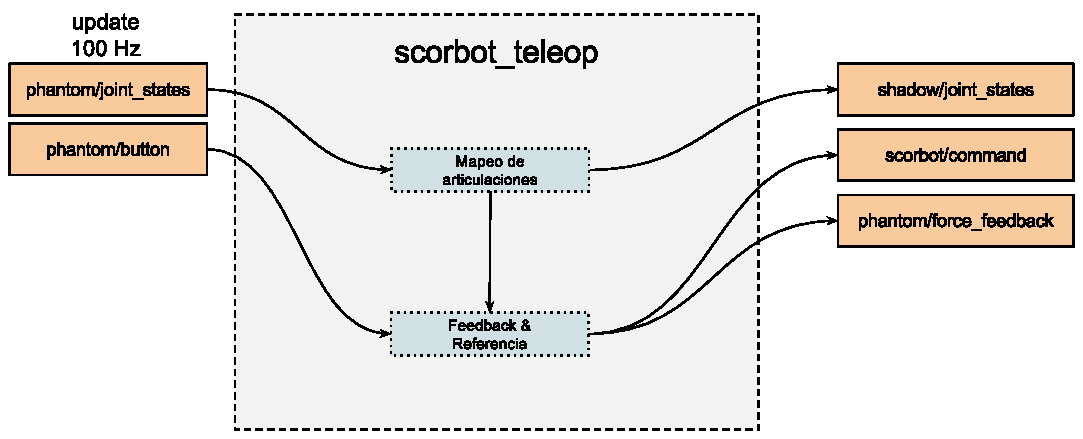
\includegraphics[width=0.8\textwidth]{img/cap4/scorbot_teleop.pdf}
  \caption{Diagrama del nodo \texttt{scorbot\_teleop}.}
  \label{cap4_scorbot_teleop}
\end{figure}

La Figura \ref{cap4_scorbot_teleop} muestra funcinamiento interno del nodo \texttt{scorbot\_teleop}, el mapeo entre el Phantom y el Scorbot \textit{shadow} se realiza de forma continua con propósitos de visualización. La retroalimentación hápica es calculada a partir de la differencia en la posición del Scorbot \textit{shadow} y el robot real, dado que ambos dispositivos tienen una morfología similar y poseen el mismo número de grados de libertad, el cálculo se realiza usando la posición de las articulaciones, como se indica en la ecuación .

\begin{equation}
F_i = K_i({X_{shadow}}_i - {X_{scorbot}}_i) \, \mbox{con } i \in {1,2,3}
\end{equation}

Notamos que el cálculo solo considera en las primeras tres articulaciones, pues el Phantom Omni solo posee estar articulaciones actuadas.

\subsubsection{Visualización}

\texttt{rviz}

\texttt{scorbot\_shadow}

\chapter{Resultados}

En este capitulo se presentan los distintos resultados de este trabajo de memoria, se presentan en un orden lógico, partiendo controladores de bajo nivel, que se ejecutan el microcontrolador; y luego, el software de control que se ejecuta en el computador.

\section{Control de articulaciones}

\subsection{Control de corriente}

El lazo de corriente corresponde al \textit{loop} de control más anidado en la estructura de control distribuido propuesta, por esta razón es la que mayor ancho de banda debe presentar (más rápido). Las pruebas de control de corriente se realizaron con el rotor bloqueado, los resultados presentatos corresponden a los obtenidos en la articulación \textit{Base}.

La Figura \ref{cap5_step_corriente} muestra la respuesta del controlador de corriente ante una entrada de tipo escalón de \SI{3}{\ampere}.

\begin{figure}[ht]
  \centering
  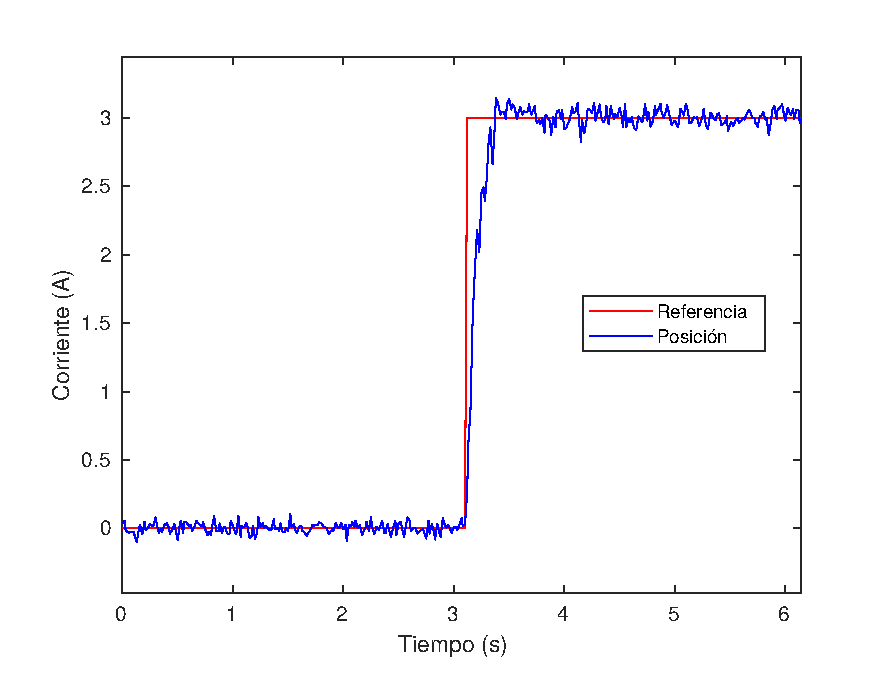
\includegraphics[width=0.5\textwidth]{img/cap5/step_corriente.pdf}
  \caption{Respuesta del controlador de corriente a un escalón.}
  \label{cap5_step_corriente}
\end{figure}

El rángo de actuación del cotrolador se há limitado a \SI{6}{\ampere}, pues corresponde a la corriente de rotor bloqueado (\textit{stall current}). La Figura \ref{cap5_corriente_cambio_referencia_alto} muestra el seguimiento de corriente a lo largo del rango de actuación durante pruebas de rotor bloqueado.

\begin{figure}[ht]
  \centering
  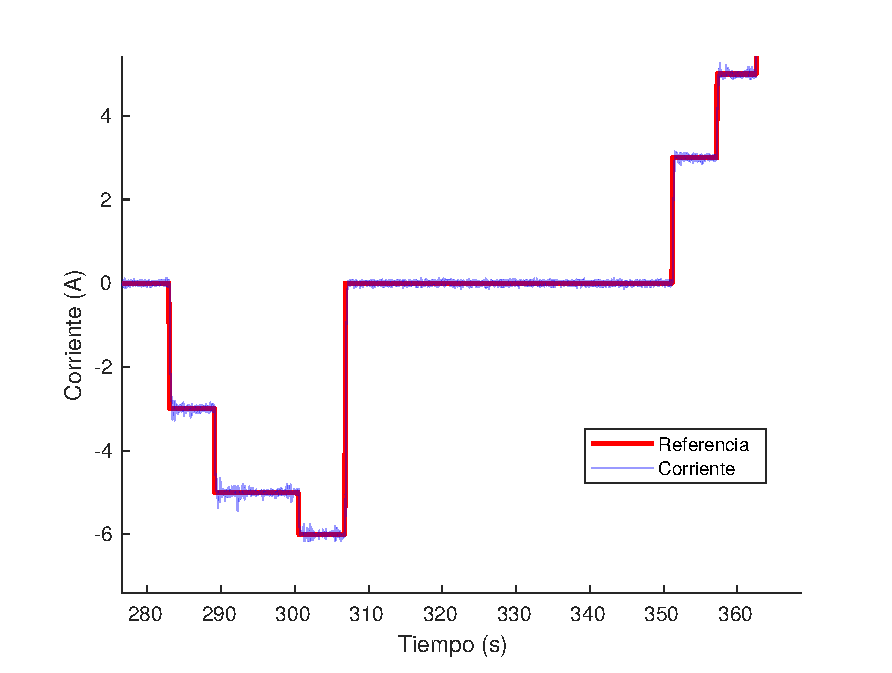
\includegraphics[width=0.5\textwidth]{img/cap5/corriente_cambio_referencia_alto.pdf}
  \caption{Respuesta del controlador de corriente ante cambios de tipo escalón en el rango completo de actuación.}
  \label{cap5_corriente_cambio_referencia_alto}
\end{figure}

Por otro lado

Seguimiento de referencia de baja amplitud
aumento del ruido por resolución del sensor
seguimiento OK

\begin{figure}[ht]
  \centering
  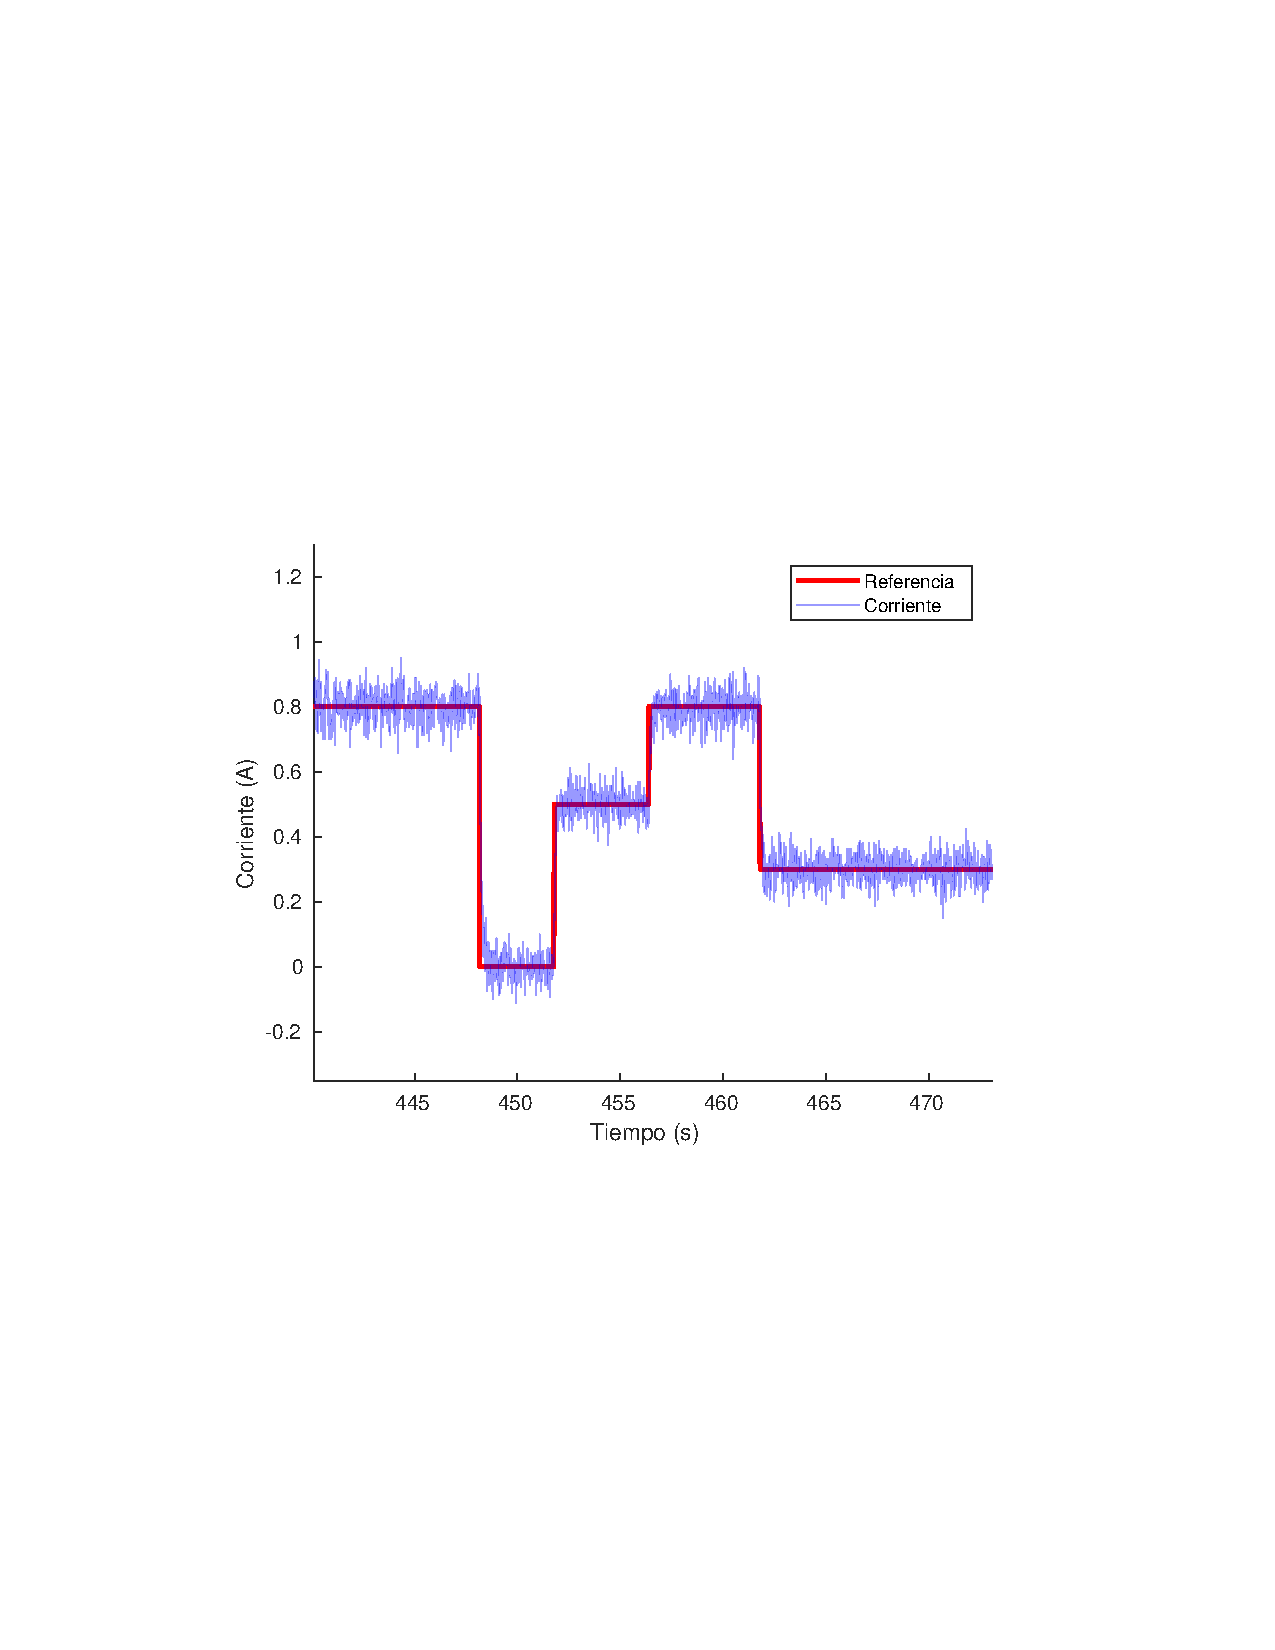
\includegraphics[width=0.5\textwidth]{img/cap5/corriente_cambio_referencia_bajo.pdf}
  \caption{Respuesta del controlador de corriente a un escalón.}
  \label{cap5_corriente_cambio_referencia_bajo}
\end{figure}




Cambio dinamico
pruebas realizadas con rotor bloqueado
movimiento induce que no se pueda alcanzar la corriente por falta de carga, antiwindup debe actuar

\begin{figure}[ht]
  \centering
  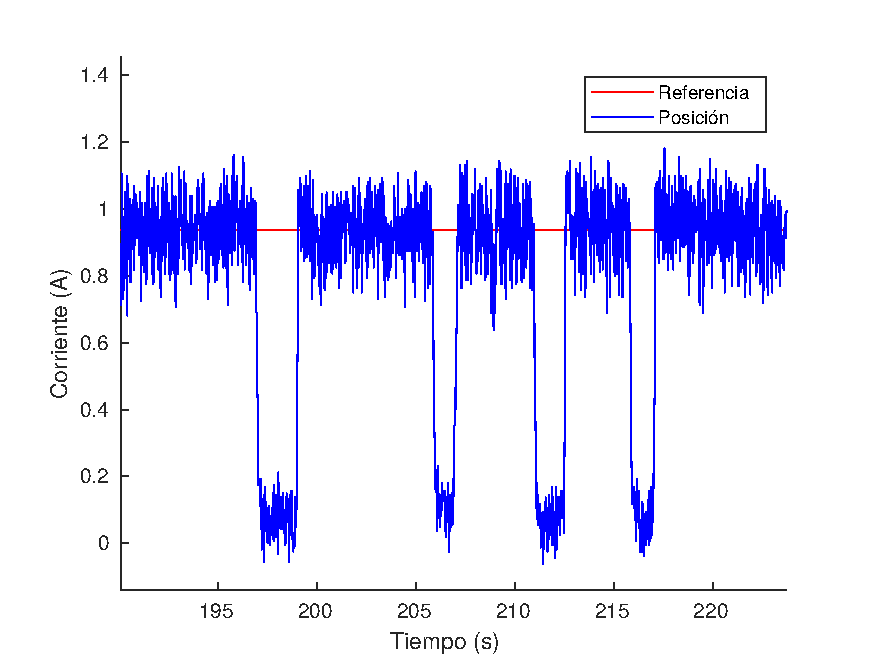
\includegraphics[width=0.5\textwidth]{img/cap5/cambio_dinamico_corriente.pdf}
  \caption{Respuesta del controlador de corriente a un escalón.}
  \label{cap5_cambio_dinamico_corriente}
\end{figure}


\subsection{Control de velocidad}

\subsection{Control de posición}

\begin{figure}[H]
  \centering
  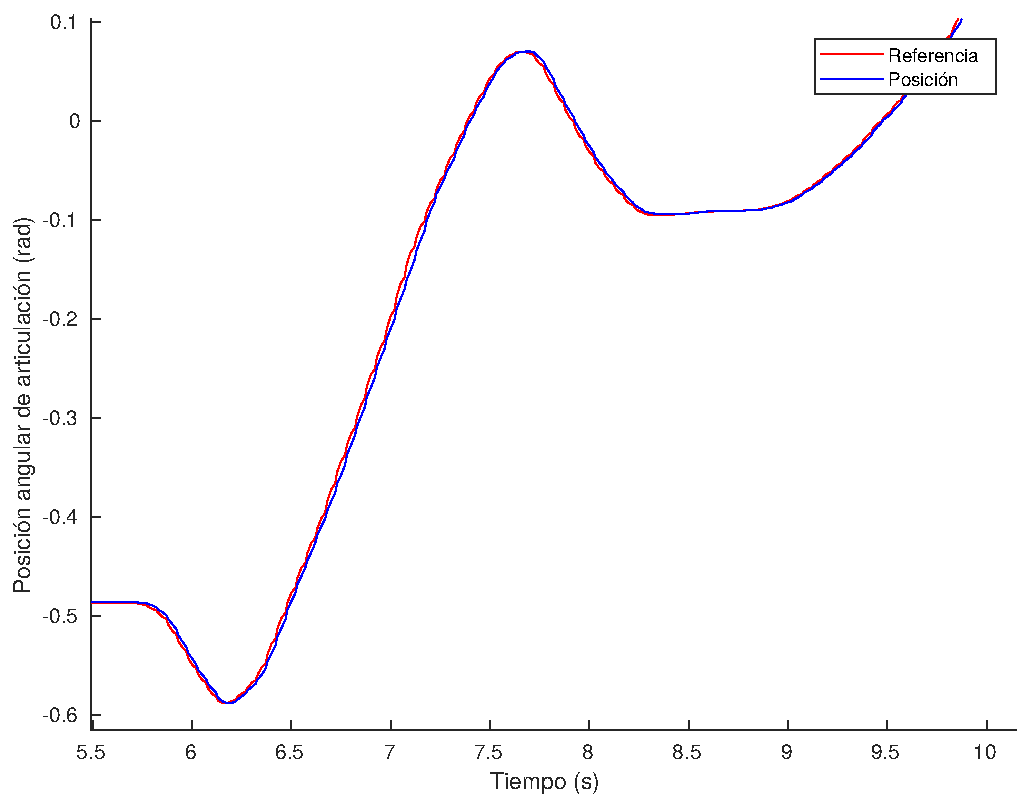
\includegraphics[width=0.5\textwidth]{img/cap5/ref_basica}
  \caption{Respuesta del controlador de corriente a un escalón.}
  \label{cap5_ref_basica}
\end{figure}



\begin{figure}[H]
  \centering
  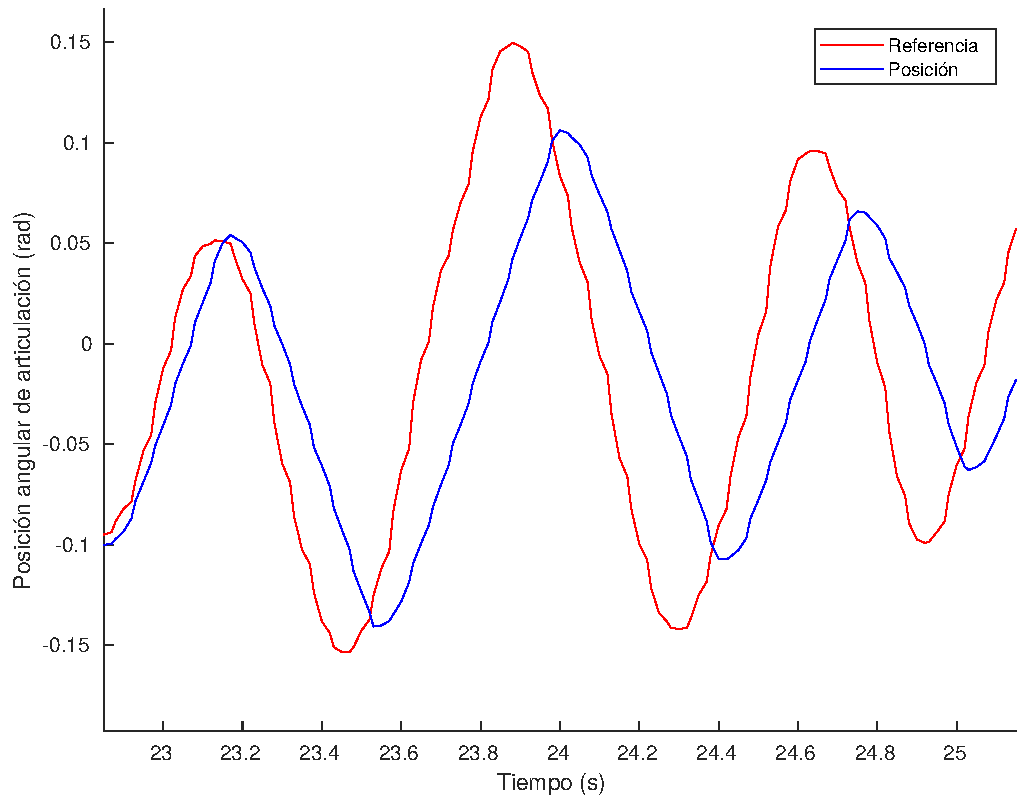
\includegraphics[width=0.5\textwidth]{img/cap5/ref_retardo_vel}
  \caption{Respuesta del controlador de corriente a un escalón.}
  \label{cap5_ref_retardo_vel}
\end{figure}

\begin{figure}[H]
  \centering
  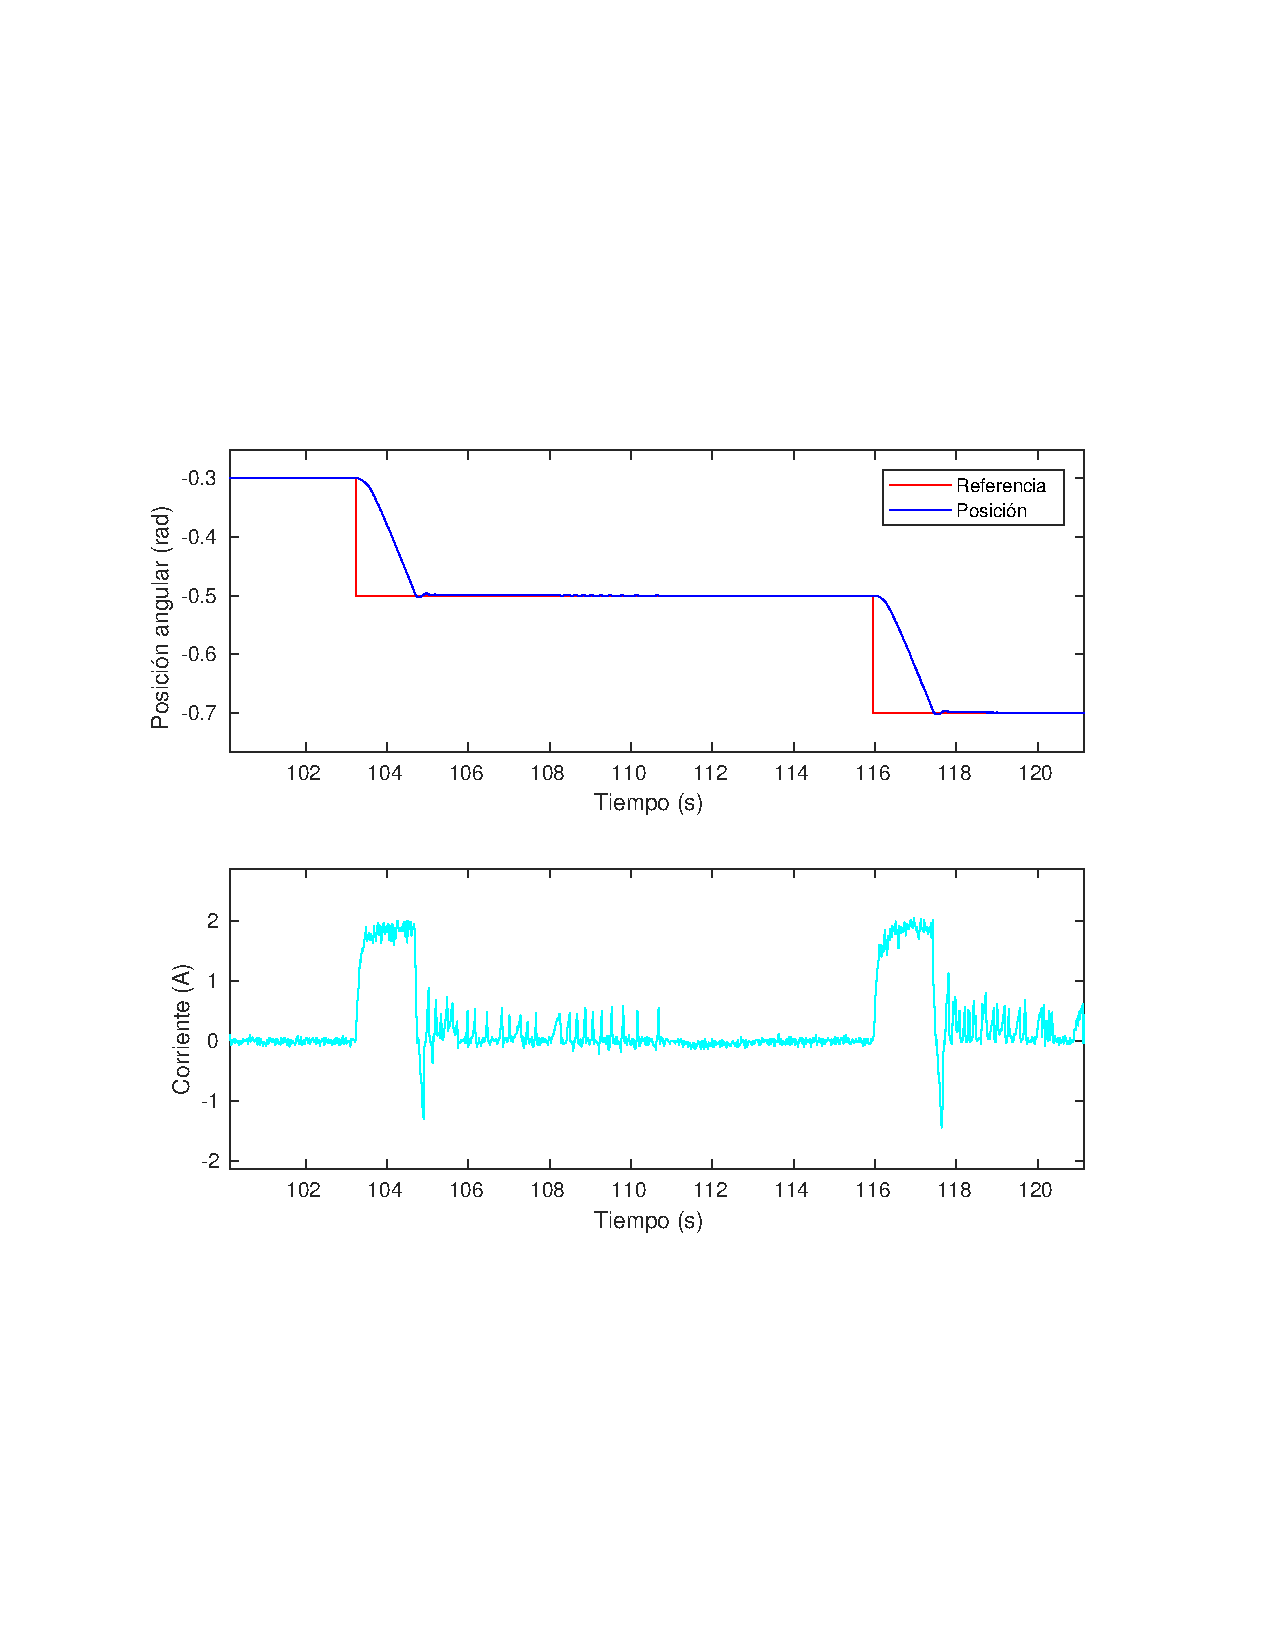
\includegraphics[width=0.8\textwidth]{img/cap5/ref_corriente_limitada}
  \caption{Respuesta del controlador de corriente a un escalón.}
  \label{cap5_ref_corriente_limitada}
\end{figure}

\section{Control mediante Phantom Omni}

\subsection{Mapeo de articulaciones}

\begin{figure}[H]
  \centering
  \begin{subfigure}[b]{0.35\textwidth}
    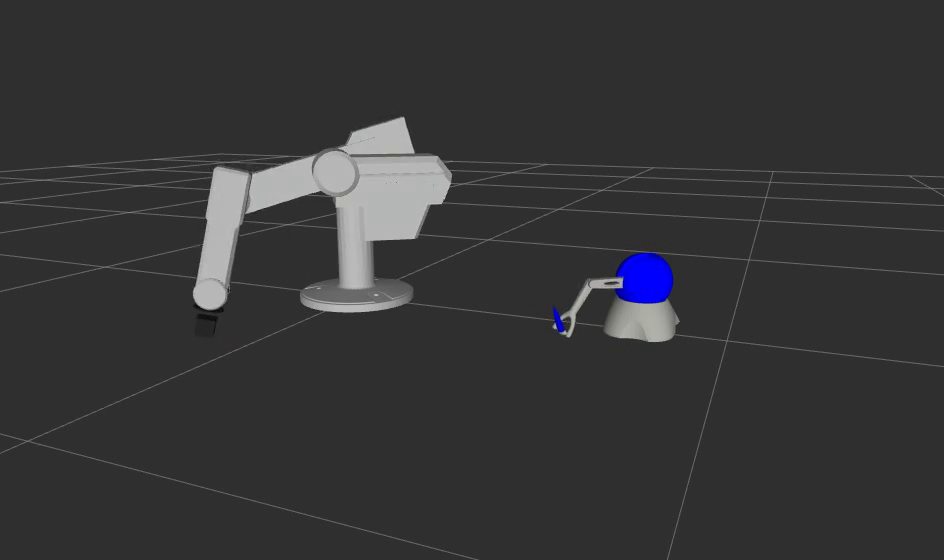
\includegraphics[width=0.9\textwidth]{img/cap5/mapping_01}
    \caption{}
  \end{subfigure}%
  \quad
  \begin{subfigure}[b]{0.35\textwidth}
    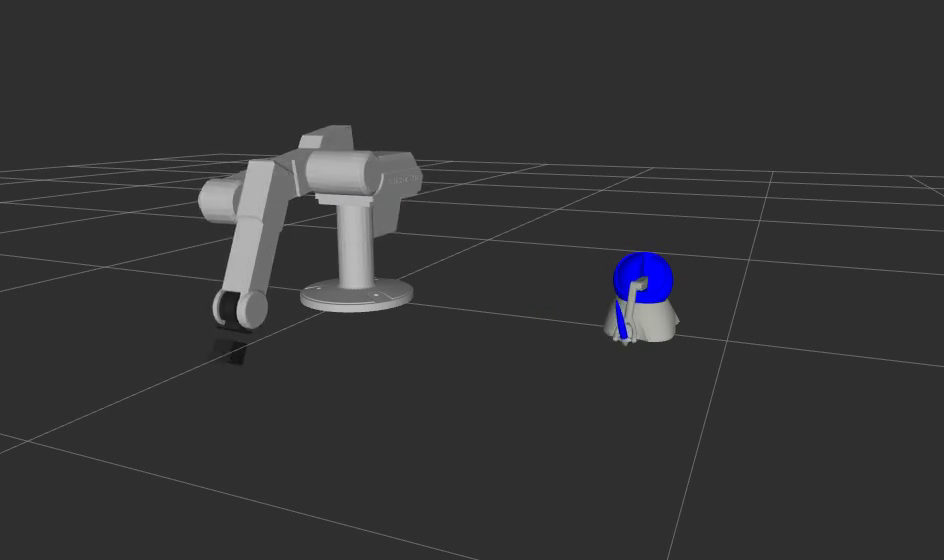
\includegraphics[width=0.9\textwidth]{img/cap5/mapping_02}
    \caption{}
  \end{subfigure}
  \vskip\baselineskip
  \begin{subfigure}[b]{0.35\textwidth}
    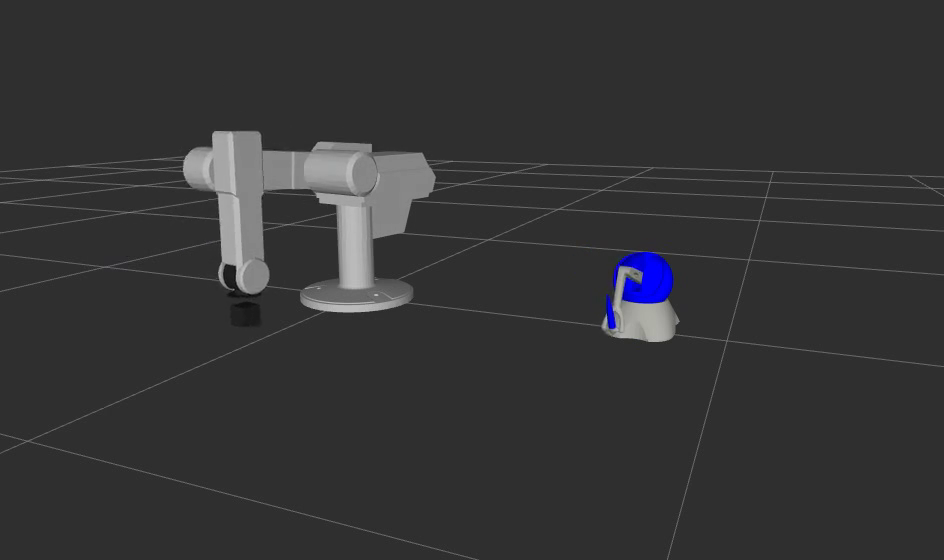
\includegraphics[width=0.9\textwidth]{img/cap5/mapping_03}
    \caption{}
  \end{subfigure}%
  \quad
  \begin{subfigure}[b]{0.35\textwidth}
    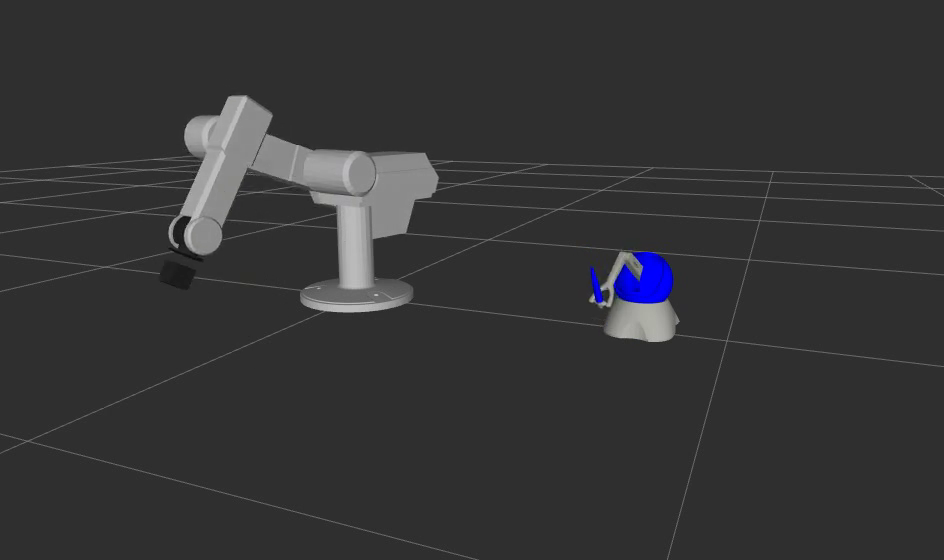
\includegraphics[width=0.9\textwidth]{img/cap5/mapping_04}
    \caption{}
  \end{subfigure}
  \caption{Mapeo de articulaciones entre el Phantom Omni y el robot Scorbot.}
  \label{cap5_joint_mapping}
\end{figure}


\subsection{Feedback haptico}

\begin{figure}[H]
  \centering
  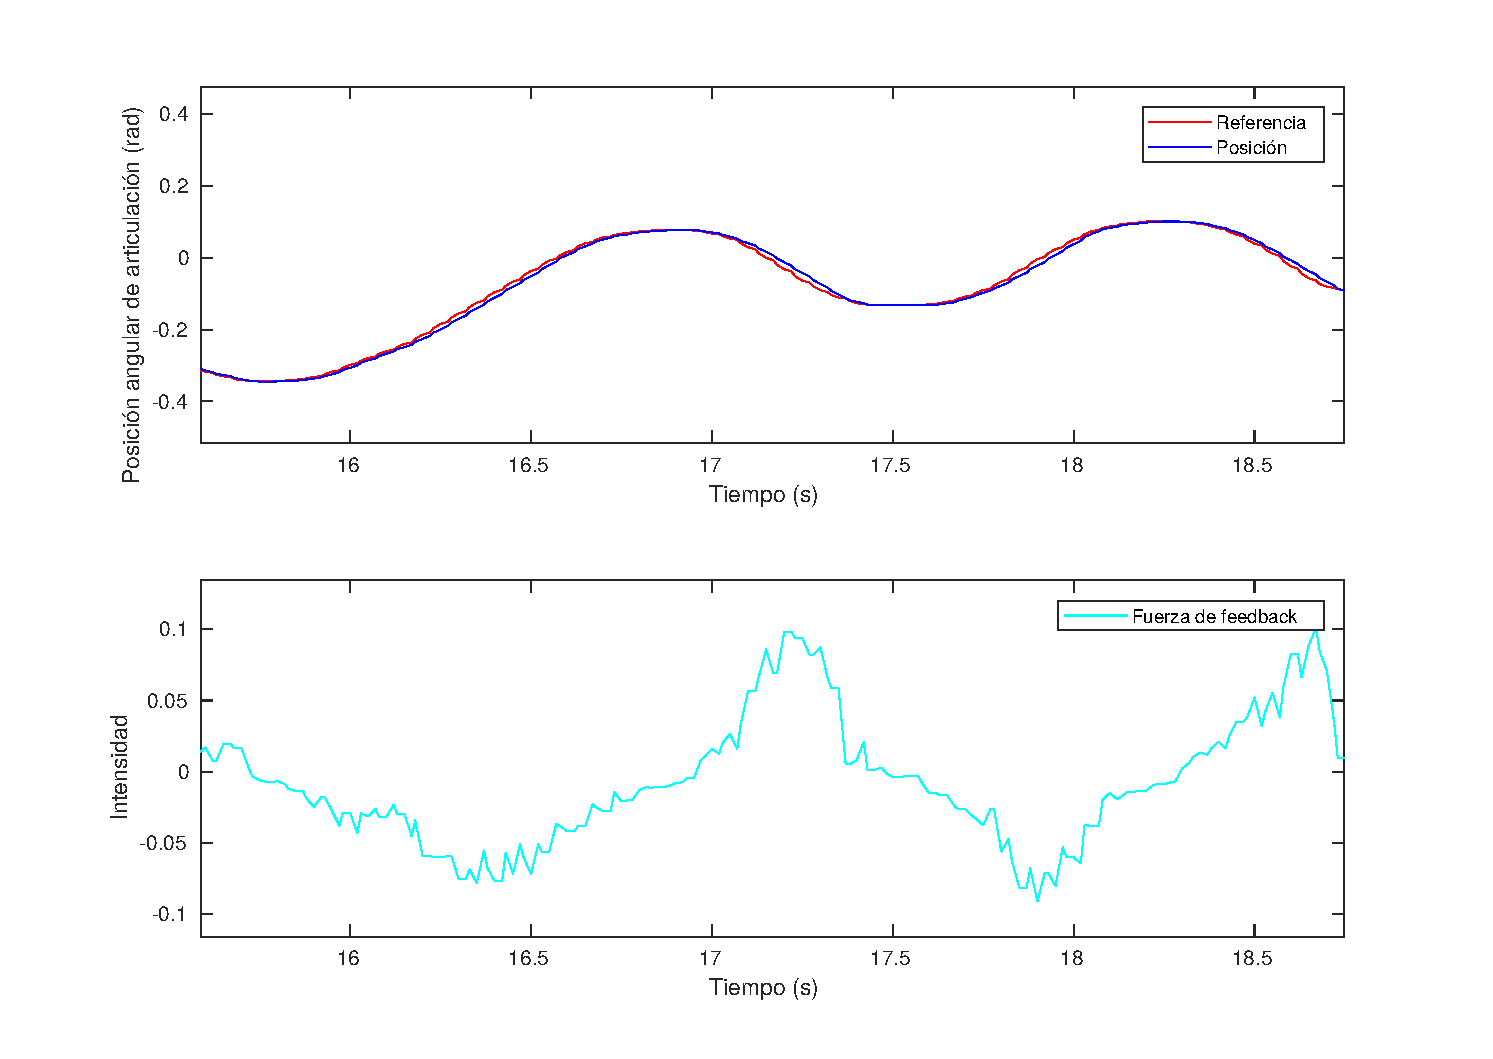
\includegraphics[width=0.5\textwidth]{img/cap5/feedback_basico}
  \caption{Algoritmo de fuerza.}
  \label{cap5_feedback_basico}
\end{figure}


\begin{figure}[H]
  \centering
  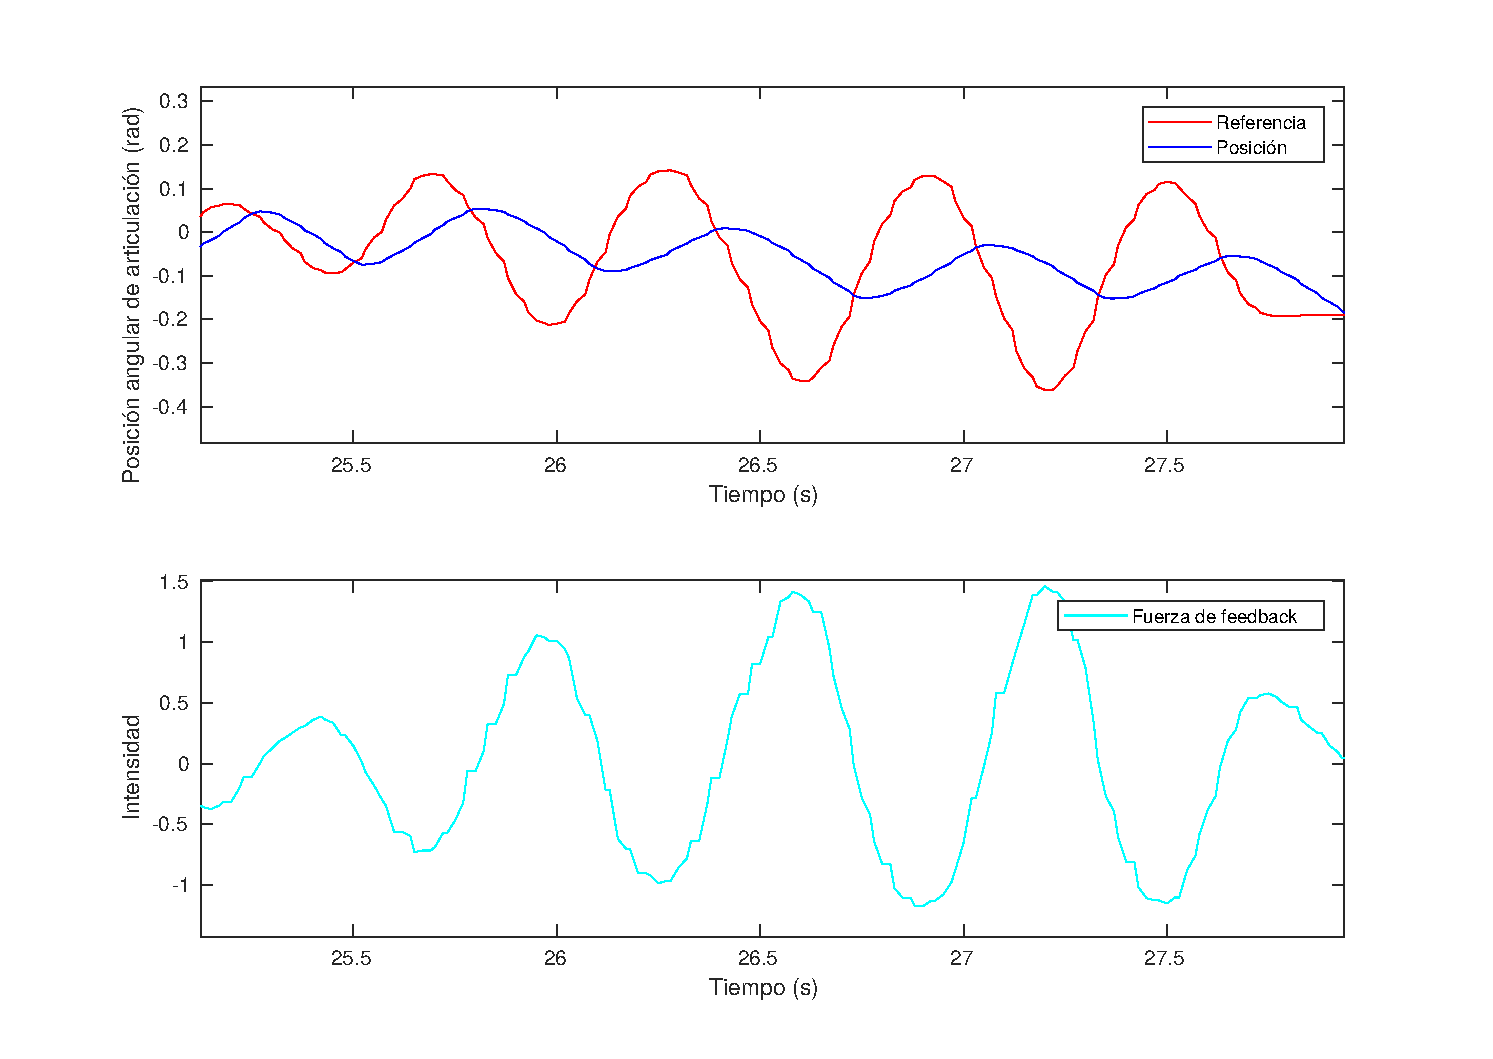
\includegraphics[width=0.5\textwidth]{img/cap5/feedback_velocidad}
  \caption{Seguimiento de trayectoria con aplicación de fuerza.}
  \label{cap4_force_tracking}
\end{figure}







\chapter{Anexos}

\begin{figure}[ht]
  \centering
  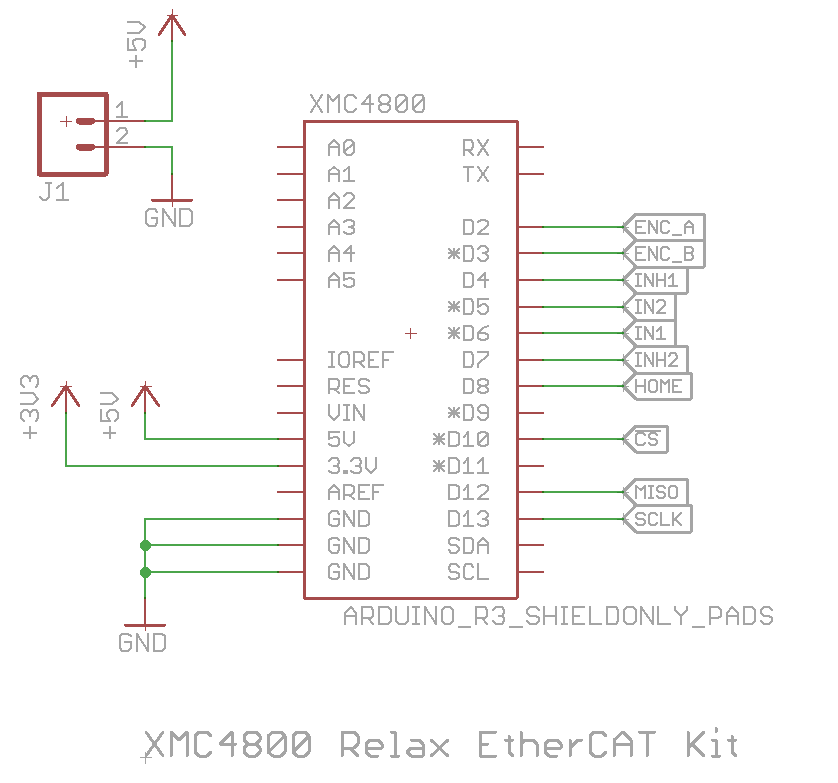
\includegraphics[width=0.5\textwidth]{img/anexo/xmc4800_schematic}
  \caption{Circuito esquemático para integración con placa de desarrollo XMC4800.}
  \label{cap4_scorbot_firmware}
\end{figure}

\begin{figure}[ht]
  \centering
  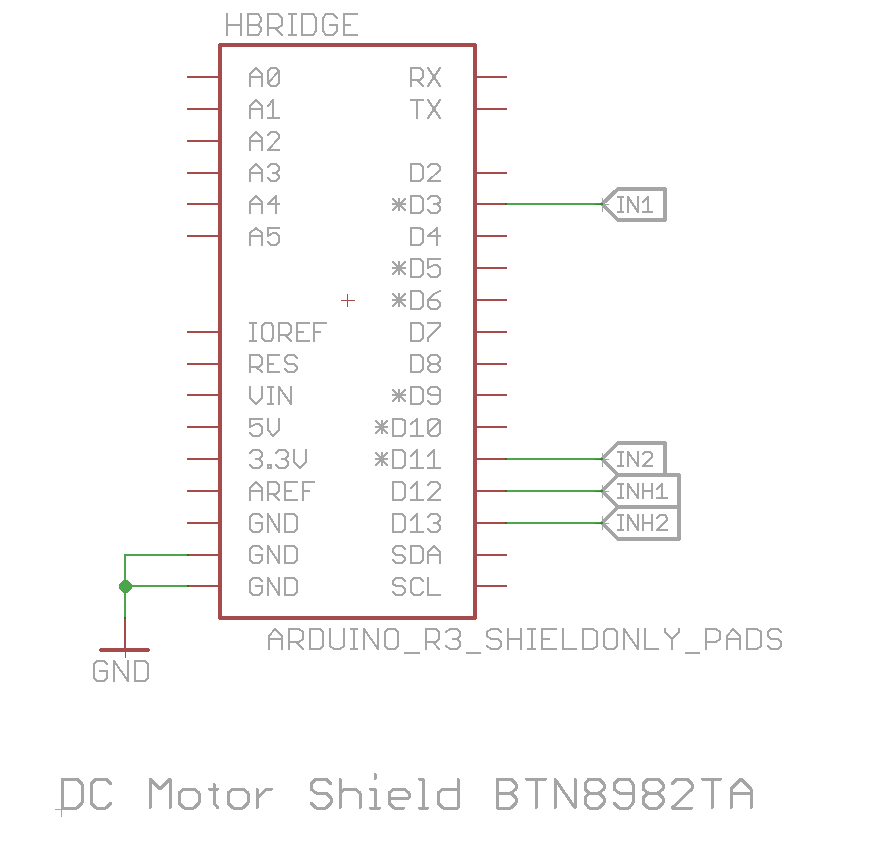
\includegraphics[width=0.5\textwidth]{img/anexo/puente_h_schematic}
  \caption{Circuito esquemático para integración con puente H.}
  \label{cap4_scorbot_firmware}
\end{figure}


\begin{figure}[ht]
  \centering
  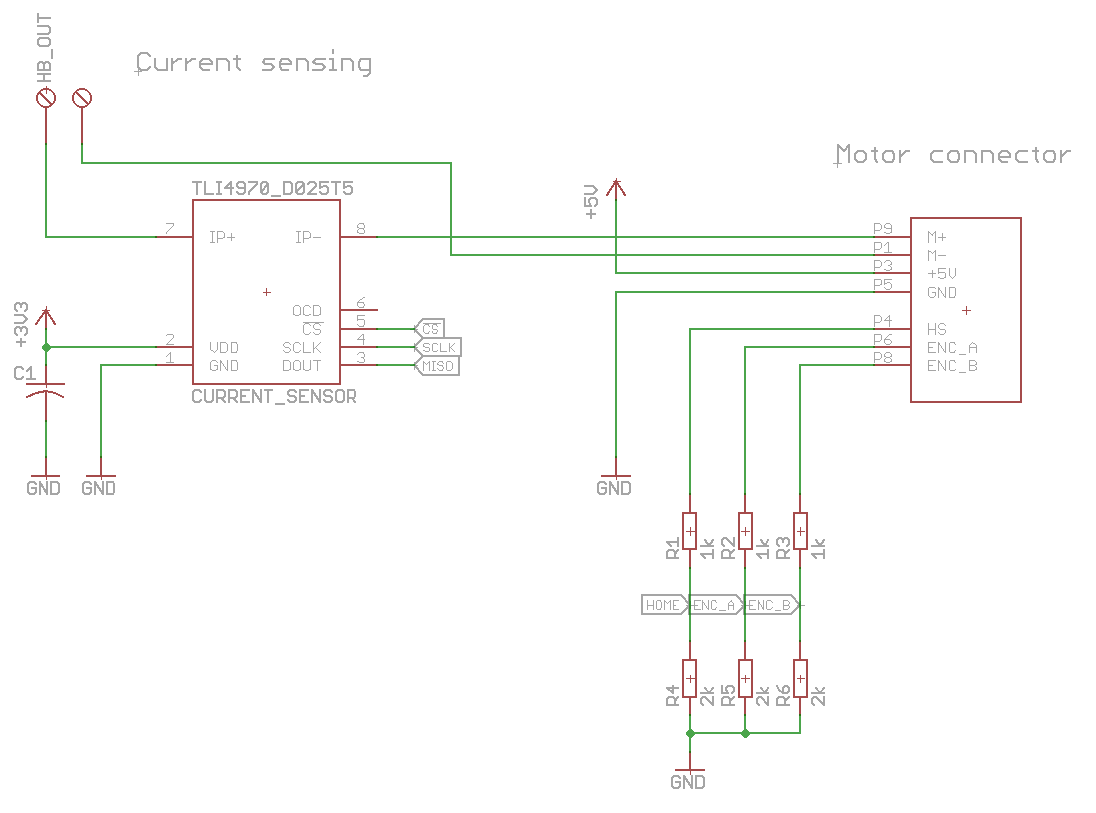
\includegraphics[width=0.5\textwidth]{img/anexo/current_sensor_schematic}
  \caption{Circuito esquemático de conexión del motor y sensor de corriente.}
  \label{cap4_scorbot_firmware}
\end{figure}


\begin{figure}[ht]
  \centering
  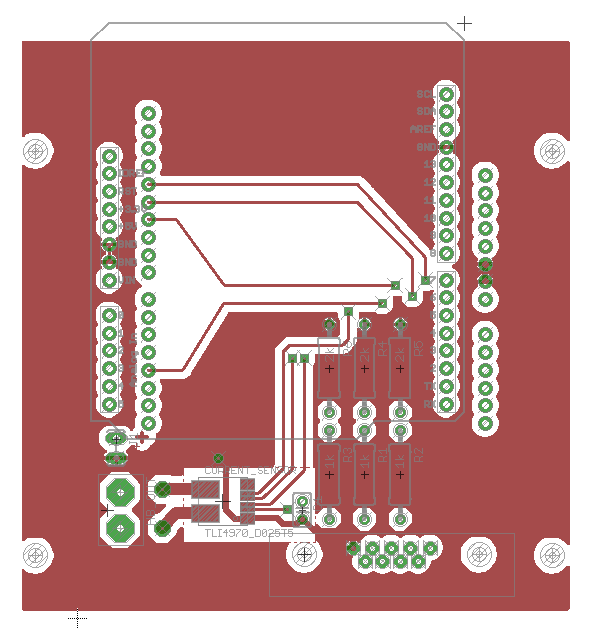
\includegraphics[width=0.5\textwidth]{img/anexo/top_layer}
  \caption{Capa superior (\textit{top}) de la placa de integración.}
  \label{cap4_scorbot_firmware}
\end{figure}


\begin{figure}[ht]
  \centering
  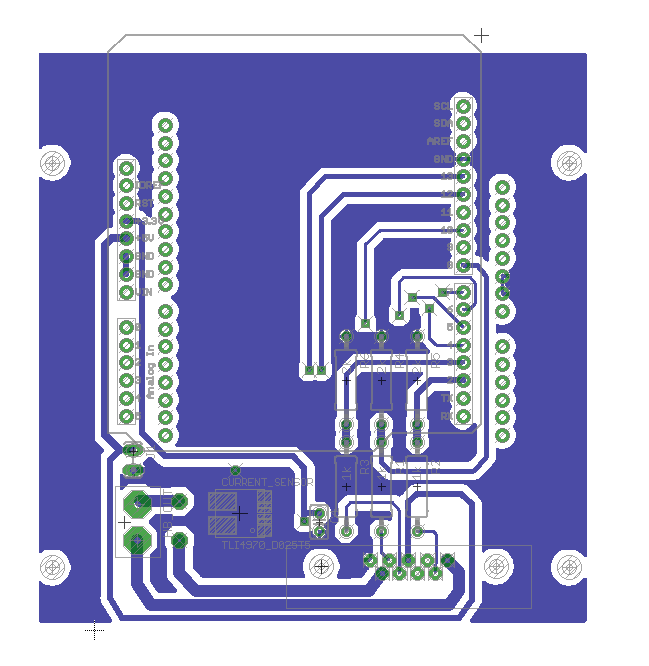
\includegraphics[width=0.5\textwidth]{img/anexo/bottom_layer}
  \caption{Capa inferior (\textit{bottom}) de la placa de integración.}
  \label{cap4_scorbot_firmware}
\end{figure}



\nocite{*}
\bibliographystyle{ieeetr}
\bibliography{bibliografia.bib}
\end{document}
